% TCC: Gerador de formas de onda por síntese digital direta em FPGA (Nicholas Seifert).
% Baseado no modelo canônico de TCC do curso de Engenharia Eletrônica da UTFPR campus Campo
% Mourão (prof. Osmar Tormena Júnior). Trechos em vermelho (\pendente) ainda dependem do autor.
%

%-----------------------------------------------------------------
% METADADOS PDF/A
%-----------------------------------------------------------------
\begin{filecontents*}{\jobname.xmpdata}
	\Author{Nicholas Seifert}
	\Title{Gerador de formas de onda por síntese digital direta em FPGA}
	\Language{pt-BR}
	\Keywords{síntese digital direta\sep FPGA\sep VHDL\sep gerador de funções\sep JTAG}
	\Publisher{RIUT}
	\Subject{Desenvolvimento de um gerador de formas de onda por síntese digital direta em FPGA, controlado por computador via Virtual JTAG, com placa analógica de saída.}
	\Copyright{Creative Commons}
	\CopyrightURL{https://creativecommons.org/licenses/by/4.0/deed.pt_BR}
	\Contributor{André Luis Régis Monteiro \sep Márcio Rodrigues da Cunha}
\end{filecontents*}

\documentclass[%
%---
% Escolha apenas uma das políticas de licenciamento
	by,				% licença CC-BY
%	by-sa,		% licença CC-BY-SA
%	by-nd,		% licença CC-BY-ND
%	by-nc,		% licença CC-BY-NC
%	by-nc-sa,	% licença CC-NC-SA
%	by-nc-nd,	% licença CC-BY-NC-ND
%---
%---
% Escolha apenas um formato de citação ABNT
%	alf	% citação (AUTOR, DATA), com referências em ordem alfabética
	num	% citação numérica, com referências na ordem de citação
%---
]{tcc-coele-cm}

%-----------------------------------------------------------------
% DADOS E CONFIGURAÇÕES PARTICULARES DO DOCUMENTO
%-----------------------------------------------------------------

%-----------------------------------------------------------------
% METADADOS DO TRABALHO
%-----------------------------------------------------------------

\author{Nicholas Seifert}
\title{Gerador de formas de onda por síntese digital direta em FPGA}
\engtitle{Direct digital synthesis waveform generator on FPGA}
\date{2026}
\advisor{André Luis Régis Monteiro, Prof.\ Dr.}
%---
% Deixe o comando \coadvisor comentado, caso não tenha co-orientador
\coadvisor{Márcio Rodrigues da Cunha, Prof.\ Dr.}
%---
% A DEFINIR: data da defesa
\approvaldate{A DEFINIR}
%---
% Membros da banca, titulação e instituição vinculada (A DEFINIR)
\boardst{MEMBRO DA BANCA A DEFINIR\\%
	Titulação\\%
	Instituição}
\boardnd{MEMBRO DA BANCA A DEFINIR\\%
	Titulação\\%
	Instituição}
\boardrd{MEMBRO DA BANCA A DEFINIR\\%
	Titulação\\%
	Instituição}
%---
	% Metadados do trabalho
%-----------------------------------------------------------------
% PACOTES DO AUTOR
%-----------------------------------------------------------------

\usepackage{multirow}	% célula em múltiplas linhas em uma tabela

%-----------------------------------------------------------------
% DEFINIÇÕES DO AUTOR
%-----------------------------------------------------------------

\newcommand{\babel}{\texttt{babel}}
\newcommand{\memoir}{\texttt{memoir}}
\newcommand{\pdflatex}{\texttt{pdflatex}}
\newcommand{\pdftex}{\texttt{pdftex}}
\newcommand{\tex}{\texttt{tex}}

%-----------------------------------------------------------------
% DEFINIÇÕES DE SIGLAS, ACRÔNIMOS E ABREVIATURAS
%-----------------------------------------------------------------

\DeclareAcronym{abnt}{%
	short=ABNT,%
	long=Associação Brasileira de Normas Técnicas%
}
\DeclareAcronym{ascii}{%
	short=ASCII,%
	long=Código Padrão Americano para o Intercâmbio de Informação,%
	foreign=\eng{American Standard Code for Information Interchange}%
}
\DeclareAcronym{coele}{%
	short=COELE-CM,%
	long=Coordenação de Engenharia Eletrônica%
}
\DeclareAcronym{ctan}{%
	short=CTAN,%
	long=Rede Compreensiva de Arquivos \TeX,%
	foreign=\eng{Comprehensive \TeX\ Archive Network}%
}
\DeclareAcronym{daeln}{%
	short=DAELN-CM,%
	long=Departamento Acadêmico de Eletrônica%
}
\DeclareAcronym{dcn}{%
	short=DCN,%
	long=Diretrizes Curriculares Nacionais%
}
\DeclareAcronym{doi}{%
	short=DOI,%
	long=Identificador de Objeto Digital,%
	foreign=\eng{Digital Object Identifier}%
}
\DeclareAcronym{dvi}{%
	short=DVI,%
	long=Independente do Dispositivo,%
	foreign=\eng{Device Independent}%
}
\DeclareAcronym{jpeg}{%
	short=JPEG,%
	long=Grupo Conjunto de Especialistas Fotográficos,%
	foreign=\eng{Joint Photographic Experts Group}%
}
\DeclareAcronym{nbr}{%
	short=NBR,%
	long=Norma Brasileira Regulamentadora%
}
\DeclareAcronym{pdf}{%
	short=PDF,%
	long=Formato de Documento Portátil,%
	foreign=\eng{Portable Document Format}%
}
\DeclareAcronym{pdfa}{%
	short=PDF/A,%
	long=Formato de Documento Portátil\slash Arquivo,%
	foreign=\eng{Portable Document Format\slash Archive}%
}
\DeclareAcronym{png}{%
	short=PNG,%
	long=Gráficos Portáteis de Rede,%
	foreign=\eng{Portable Network Graphics}%
}
\DeclareAcronym{pratcc}{%
	short=PRATCC,%
	long=Professor Responsável pelo Trabalho de Conclusão de Curso%
}
\DeclareAcronym{riut}{%
	short=RIUT,%
	long=Repositório Institucional da UTFPR%
}
\DeclareAcronym{tcc}{%
	short=TCC,%
	long=Trabalho de Conclusão de Curso%
}
\DeclareAcronym{tug}{%
	short=TUG,%
	long=Grupo de Usuários do \TeX,%
	foreign=\TeX\ \eng{Users Group}%
}
\DeclareAcronym{utf8}{%
	short=UTF-8,%
	long=Formato Unicode de Transformação: 8 bits,%
	foreign=\eng{Unicode Transformation Format: 8-bit}%
}
\DeclareAcronym{utfpr}{%
	short=UTFPR-CM,%
	long=Universidade Tecnológica Federal do Paraná campus Campo Mourão%
}

	% Pacotes adicionais e macros do autor

%-----------------------------------------------------------------
% ARQUIVO DE REFERÊNCIAS
%-----------------------------------------------------------------

\addbibresource{./postextual/refs.bib}

%-----------------------------------------------------------------
% INÍCIO DO DOCUMENTO
%-----------------------------------------------------------------

\begin{document}

%-----------------------------------------------------------------
% PARTE EXTERNA
%-----------------------------------------------------------------

\maketitle	% Capa

%-----------------------------------------------------------------
% PARTE INTERNA
%-----------------------------------------------------------------

%-----------------------------------------------------------------
% ELEMENTOS PRÉ-TEXTUAIS
%-----------------------------------------------------------------

\frontmatter
\maketitlepage		% Folha de rosto
\approval			% Folha de aprovação
\dedication			% Dedicatória (opcional)
\acknowledgment		% Agradecimentos (opcional)
\printepigraph		% Epígrafe (opcional)
\printabstract		% Resumo
\printengabstract	% Abstract
\printlof			% Lista de figuras (opcional)
\printlot			% Lista de tabelas (opcional)
\printloa			% Lista de acrônimos e siglas (opcional)
\printtoc			% Sumário

%-----------------------------------------------------------------
% ELEMENTOS TEXTUAIS
%-----------------------------------------------------------------

\mainmatter
\acresetall	% siglas por extenso de novo na primeira vez que aparecem no texto
\chapter{Introdução}

Geradores de sinais estão entre os instrumentos mais usados em um laboratório de eletrônica: alimentam circuitos sob teste com senoides, rampas e pulsos de frequência e amplitude conhecidas. Os geradores de funções e de formas de onda arbitrárias atuais são, em sua maioria, digitais. Em vez de um oscilador analógico, eles calculam as amostras do sinal e as convertem em tensão por meio de um \ac{dac}.

A técnica que viabiliza esses instrumentos é a \ac{dds}, descrita por \textcite{tierney1971}. Um acumulador de fase soma, a cada ciclo de clock, um valor constante chamado palavra de sintonia; a fase acumulada endereça uma tabela que contém um período da forma de onda; e o \ac{dac} converte as amostras lidas em um sinal analógico, que um filtro passa-baixas suaviza. A frequência de saída é proporcional à palavra de sintonia, o que dá à \ac{dds} resolução de frequência muito fina, troca de frequência sem descontinuidade de fase e formas de onda definidas apenas pelo conteúdo de uma tabela \cites{ad1999,kester2008}.

Os \acp{fpga} são adequados para implementar a \ac{dds}: oferecem memória interna para as tabelas, multiplicadores dedicados, \acp{pll} para gerar o clock e lógica suficiente para acrescentar interfaces de controle. O curso de Engenharia Eletrônica da \ac{utfpr} dispõe da placa de desenvolvimento DE2-115, com um \ac{fpga} Cyclone IV E, que reúne esses recursos \cite{terasic2010}.

Este trabalho apresenta o desenvolvimento de um gerador de formas de onda por \ac{dds} completo, do código em \ac{vhdl} ao conector de saída. O núcleo digital roda no \ac{fpga} da DE2-115 e é controlado pelo computador através do próprio cabo de gravação da placa, usando o recurso Virtual \ac{jtag} da Intel. Uma placa analógica própria converte as amostras em tensão, com um \ac{dac} de 8~bits, um filtro de reconstrução e ajuste de amplitude. Uma interface gráfica em Python permite escolher a frequência, a forma de onda e o conteúdo de uma tabela arbitrária.

Os capítulos seguintes estão organizados da seguinte forma: o Capítulo~\ref{cap:teoria} apresenta a fundamentação teórica da \ac{dds}, dos \acp{fpga} e dos circuitos analógicos de saída; o Capítulo~\ref{cap:metodologia} descreve o projeto do sistema, do núcleo digital, da verificação por simulação, da interface com o usuário e da placa analógica; o Capítulo~\ref{cap:resultados} apresenta e discute os resultados de síntese, de simulação e de bancada; e o Capítulo~\ref{cap:conclusao} reúne as conclusões e as propostas de trabalhos futuros.

\section{Objetivos}

O objetivo principal deste trabalho é desenvolver um gerador de formas de onda por síntese digital direta, implementado em \ac{fpga} e controlado por computador, capaz de gerar senoides, rampas, funções sinc e formas arbitrárias com frequência de 0 a 262\,143~Hz e resolução de 2,33~mHz.

Os objetivos específicos podem ser discriminados como:
\begin{itemize}
	\item Implementar em \ac{vhdl} um núcleo \ac{dds} com acumulador de fase de 32~bits, tabelas de 1024~amostras de 8~bits e conversão da frequência em hertz para a palavra de sintonia sem o uso de divisores;
	\item Implementar o controle pelo computador através do Virtual \ac{jtag}, incluindo a passagem segura dos comandos entre domínios de clock e a escrita da forma arbitrária com o gerador em operação;
	\item Organizar o projeto digital em blocos encapsulados, cada um com interface bem definida, e verificar cada bloco por simulação com \eng{testbenches} auto-verificáveis;
	\item Projetar a placa analógica de saída, com \ac{dac}, conversão corrente-tensão, filtro de reconstrução e ajuste de amplitude, e avaliá-la por simulação SPICE;
	\item Desenvolver uma interface gráfica para configurar a frequência, a forma de onda e a tabela arbitrária;
	\item Validar o sistema completo em bancada.
\end{itemize}

\section{Justificativa}

O presente trabalho se justifica pelos seguintes critérios:
\begin{description}
	\item[Didática] --- em um gerador comercial, o funcionamento interno fica oculto. No sistema desenvolvido, cada etapa da \ac{dds} (acumulação de fase, truncamento, quantização, conversão e reconstrução) pode ser observada, medida e modificada, o que o torna útil para o ensino de processamento digital de sinais e de conversão de dados;
	\item[Flexibilidade] --- como a forma de onda é apenas o conteúdo de uma tabela, o gerador pode reproduzir sinais que um gerador de funções comum não oferece, como o eletrocardiograma sintético usado neste trabalho para testar equipamentos biomédicos;
	\item[Aproveitamento de recursos] --- o sistema usa a placa DE2-115, já disponível no curso, e o controle pelo computador dispensa qualquer hardware além do cabo de gravação. A placa analógica usa componentes comuns, como o \ac{dac} DAC0800 e o amplificador operacional TL074;
	\item[Integração] --- o trabalho reúne projeto digital, projeto analógico, desenvolvimento de software e verificação, competências distribuídas ao longo da formação em Engenharia Eletrônica.
\end{description}

\chapter{Fundamentação teórica}\label{cap:teoria}

Neste capítulo são apresentados os conceitos em que o trabalho se apoia: o princípio da síntese digital direta e suas fontes de erro; os dispositivos lógicos programáveis, a linguagem \ac{vhdl} e o acesso por \ac{jtag}; e os circuitos analógicos que convertem as amostras digitais em tensão. O leitor interessado pode aprofundar os conceitos através das referências.

\section{Síntese digital direta}

A \ac{dds} gera um sinal periódico a partir de um clock de referência de frequência fixa, \(f_{clk}\). A arquitetura clássica, mostrada na Figura~\ref{fig:dds_blocos}, tem quatro blocos: um acumulador de fase de \(N\)~bits, que avança um passo \(M\) a cada clock; um truncamento, que aproveita apenas os \(P\)~bits mais significativos da fase; uma \ac{lut}, que converte a fase em amplitude com \(D\)~bits; e um \ac{dac} seguido de um filtro passa-baixas, que reconstroem o sinal analógico \cites{tierney1971,ad1999,vankka2001}.

\begin{figure}
	\caption{Arquitetura clássica de um sintetizador digital direto e o sinal em cada ponto.}
	\label{fig:dds_blocos}
	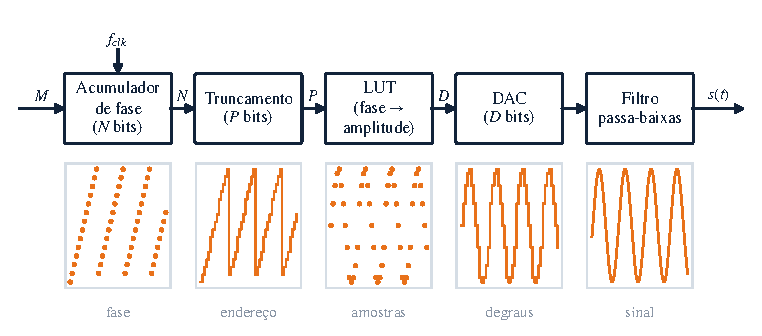
\includegraphics[width=\textwidth]{./figuras/dds_blocos}
	\legend{Fonte~---~Autoria própria.}
\end{figure}

\subsection{Acumulador de fase}

O acumulador de fase é um somador de \(N\)~bits cuja saída é registrada e realimentada. A cada borda do clock, ele soma ao valor atual a palavra de sintonia \(M\), também chamada de \ac{ftw}:
\begin{equation}\label{eq:acumulador}
	\phi[k] = \left(\phi[k-1] + M\right) \bmod 2^{N}.
\end{equation}
O valor \(\phi[k]\) representa a fase do sinal: os \(2^N\) estados do registrador correspondem a uma volta completa, de 0 a \(2\pi\). O estouro natural do somador, que descarta o vai-um, realiza a operação módulo sem nenhuma lógica adicional. Como a fase avança \(M\) estados por clock, uma volta leva \(2^N/M\) clocks, e a frequência de saída é
\begin{equation}\label{eq:fout}
	f_{out} = \frac{M \cdot f_{clk}}{2^{N}}.
\end{equation}

A menor variação de frequência possível, a resolução do gerador, corresponde a \(M = 1\):
\begin{equation}\label{eq:resolucao}
	\Delta f = \frac{f_{clk}}{2^{N}}.
\end{equation}
Com \(N = 32\) e \(f_{clk} = 10\)~MHz, \(\Delta f \approx 2{,}33\)~mHz. Essa resolução fina com um clock fixo é a principal vantagem da \ac{dds} sobre as técnicas baseadas em \ac{pll} \cite{goldberg1999}.

A Figura~\ref{fig:roda_fase} ilustra o acumulador como uma roda: com \(N = 8\), a roda tem 256 estados, e o ponteiro avança \(M = 40\) estados a cada clock. Como 256 não é múltiplo de 40, uma volta leva 6,4 clocks, e as amostras caem em posições diferentes a cada período; ainda assim, o período médio é exatamente o dado pela Equação~(\ref{eq:fout}). Quando \(M\) muda, o acumulador continua a partir da fase em que estava, de modo que a troca de frequência não produz salto de fase. Pelo teorema da amostragem, o passo deve satisfazer \(M < 2^{N-1}\), ou seja, \(f_{out} < f_{clk}/2\); acima disso, o sinal amostrado aparece com frequência \(f_{clk} - f_{out}\), fenômeno conhecido como \eng{aliasing} \cite{oppenheim2010}.

\begin{figure}
	\caption{Roda de fase de um acumulador de 8~bits com \(M = 40\) e tabela de 16 posições: à esquerda, as primeiras posições do ponteiro; à direita, as amostras resultantes.}
	\label{fig:roda_fase}
	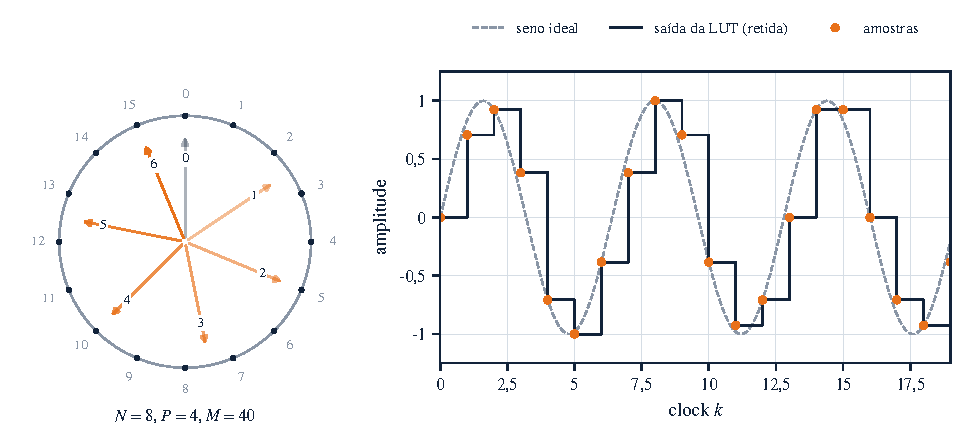
\includegraphics[width=\textwidth]{./figuras/roda_fase}
	\legend{Fonte~---~Autoria própria.}
\end{figure}

\subsection{Conversão de fase em amplitude}

A conversão de fase em amplitude é feita por uma tabela que guarda um período da forma de onda, com \(2^P\) amostras de \(D\)~bits. Para uma senoide em código binário deslocado, o conteúdo da posição \(n\) é
\begin{equation}\label{eq:lut_seno}
	x[n] = \operatorname{round}\!\left(2^{D-1} + \left(2^{D-1}-1\right)\sin\frac{2\pi n}{2^{P}}\right),
\end{equation}
de forma que o zero do sinal corresponde ao código \(2^{D-1}\). Como a tabela pode conter qualquer sequência, a mesma arquitetura gera rampas, pulsos ou formas arbitrárias. Para senoides, há técnicas que reduzem o tamanho da tabela explorando a simetria do seno, guardando apenas um quarto de período, ou que substituem a tabela por aproximações polinomiais ou pelo algoritmo CORDIC \cite{vankka2001}. Neste trabalho a tabela completa é usada, pois a memória do \ac{fpga} é suficiente e a mesma estrutura atende às formas arbitrárias.

A amostra de \(D\)~bits introduz um erro de quantização de amplitude. Para uma senoide de escala completa, considerando o erro como ruído uniforme, a \ac{snr} máxima é \cite{kester2005}
\begin{equation}\label{eq:snr}
	\mathrm{SNR} \approx 6{,}02\,D + 1{,}76~\text{dB},
\end{equation}
que resulta em cerca de 50~dB para \(D = 8\).

\subsection{Truncamento de fase e espúrios}

Uma tabela com \(2^{N}\) posições seria inviável: com \(N = 32\), seriam mais de quatro bilhões de amostras. Por isso, apenas os \(P\)~bits mais significativos da fase endereçam a tabela, e os \(N-P\) bits restantes são descartados. Os bits descartados continuam acumulando, de modo que a frequência média permanece correta, mas a fase usada para endereçar a tabela tem um erro periódico. Esse erro modula a fase do sinal de saída e aparece no espectro como componentes espúrias discretas. No pior caso, a \ac{sfdr}, distância entre a portadora e o maior espúrio, é aproximadamente \cites{nicholas1987,vankka2001}
\begin{equation}\label{eq:sfdr}
	\mathrm{SFDR} \approx 6{,}02\,P~\text{dBc}.
\end{equation}

A Figura~\ref{fig:espectros}(a) mostra o espectro das amostras de um \ac{dds} com \(N = 32\), \(P = 10\) e \(D = 8\), os parâmetros deste trabalho, obtido por simulação numérica com \ac{fft} de \(2^{16}\) pontos e janela de Blackman. O maior espúrio fica 60,1~dB abaixo da portadora, em acordo com a Equação~(\ref{eq:sfdr}), que prevê 60,2~dB para \(P = 10\). O piso de ruído, abaixo dos espúrios, vem da quantização de amplitude.

\begin{figure}
	\caption{(a) Espectro das amostras de um \acs{dds} com \(N = 32\), \(P = 10\) e \(D = 8\), obtido por simulação numérica; (b) saída de um \acs{dac} com retenção de ordem zero: imagens em torno dos múltiplos de \(f_{clk}\), envoltória sinc e efeito do filtro de reconstrução usado neste trabalho.}
	\label{fig:espectros}
	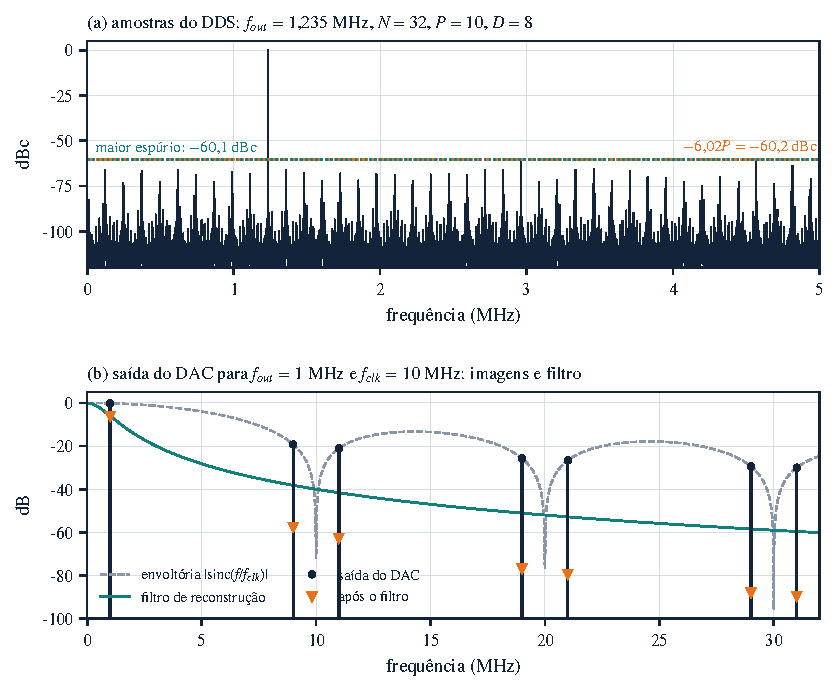
\includegraphics[width=\textwidth]{./figuras/espectros}
	\legend{Fonte~---~Autoria própria.}
\end{figure}

\subsection{Conversão digital-analógica e reconstrução}

O \ac{dac} mantém cada amostra na saída durante um período de clock, comportando-se como um \ac{zoh}. O sinal resultante é uma escada, cujo espectro contém, além da componente em \(f_{out}\), imagens em \(k f_{clk} \pm f_{out}\), para todo inteiro \(k \geq 1\). Todas as componentes são ponderadas pela resposta do retentor \cites{kester2005,oppenheim2010}:
\begin{equation}\label{eq:zoh}
	\left|H_{\mathrm{ZOH}}(f)\right| = \left|\frac{\sin(\pi f/f_{clk})}{\pi f/f_{clk}}\right|.
\end{equation}
A Equação~(\ref{eq:zoh}) mostra que a própria componente desejada é atenuada à medida que se aproxima de \(f_{clk}/2\): em \(f_{out} = f_{clk}/2\), a perda é de 3,9~dB. Para frequências bem abaixo de \(f_{clk}\), a atenuação é desprezível.

O filtro de reconstrução é um passa-baixas que deixa passar \(f_{out}\) e atenua as imagens. Quanto mais próximo \(f_{out}\) estiver de \(f_{clk}/2\), mais próxima a primeira imagem fica da banda útil e mais seletivo o filtro precisa ser. A Figura~\ref{fig:espectros}(b) mostra esse efeito para \(f_{out} = 1\)~MHz e \(f_{clk} = 10\)~MHz, com o filtro de segunda ordem usado neste trabalho.

\section{Dispositivos lógicos programáveis}

\subsection{FPGA e a família Cyclone IV E}

Um \ac{fpga} é um circuito integrado cuja função lógica é definida após a fabricação, por configuração. Na família Cyclone IV E, da Intel, o recurso básico é o \ac{le}, composto por uma tabela de quatro entradas, que implementa qualquer função combinacional dessas entradas, e por um registrador programável. Além dos \acp{le}, o dispositivo oferece blocos de memória M9K, de 9\,216~bits cada, que podem ser configurados como \ac{rom} ou como \ac{ram} de uma ou duas portas; multiplicadores dedicados de \(18 \times 18\)~bits, que também operam como dois de \(9 \times 9\); e \acp{pll}, que geram clocks com frequência múltipla ou submúltipla da referência \cite{intel2016cyclone}.

A placa DE2-115, da Terasic, usa o EP4CE115F29C7, com 114\,480 \acp{le}, 432 blocos M9K (3\,981\,312~bits de memória), 266 multiplicadores de \(18 \times 18\)~bits e quatro \acp{pll}. A placa oferece um oscilador de 50~MHz, botões com circuito de \eng{debounce}, \eng{LEDs}, um conector de expansão de 40 pinos com \ac{gpio} e um gravador USB-Blaster integrado, acessível pela porta \ac{usb} \cite{terasic2010}.

\subsection{VHDL e fluxo de projeto}

O \ac{vhdl} é uma linguagem de descrição de hardware padronizada pelo IEEE \cite{ieee2009vhdl}. Um projeto em \ac{vhdl} é organizado em entidades, que declaram as portas de um bloco, e arquiteturas, que descrevem seu comportamento ou sua estrutura. Uma arquitetura estrutural instancia outras entidades e as liga por sinais, o que permite construir o sistema de forma hierárquica, com cada bloco encapsulado atrás de sua interface \cite{pedroni2010}.

O mesmo código \ac{vhdl} tem dois usos. Na síntese, uma ferramenta como o Quartus Prime traduz a descrição em \acp{le}, memórias e conexões do \ac{fpga} e verifica se os caminhos entre registradores cumprem os requisitos de tempo do clock. Na simulação, um simulador como o GHDL executa a descrição em um computador, dentro de um \eng{testbench}: uma entidade sem portas que gera os estímulos, observa as saídas e, quando é auto-verificável, compara o resultado com um modelo de referência \cites{pedroni2010,ghdl2025}.

Funções comuns são oferecidas pelo fabricante como blocos de \ac{ip}, configurados por assistentes. Neste trabalho são usados o \cod{altsyncram}, que implementa memórias nos blocos M9K \cite{intel2018ram}, e o \cod{altpll}, que configura um \ac{pll} \cite{intel2017pll}. Ambos têm modelos de simulação em \ac{vhdl} distribuídos com o Quartus.

\subsection{JTAG e Virtual JTAG}

O padrão IEEE 1149.1, conhecido como \ac{jtag}, define uma \ac{tap} serial, com os sinais TCK, TMS, TDI e TDO, controlada por uma máquina de estados. Duas sequências de estados são usadas para acessar o dispositivo: a do registrador de instrução (IR), que escolhe qual registrador de dados será acessado, e a do registrador de dados (DR). No acesso ao DR, o estado Capture-DR carrega um valor no registrador; o Shift-DR desloca os bits, um por clock, entrando por TDI e saindo por TDO; e o Update-DR aplica o valor deslocado \cite{ieee2013jtag}.

Nos \acp{fpga} da Intel, a mesma porta \ac{jtag} usada para a gravação pode ser compartilhada com a lógica do usuário. O bloco Virtual \ac{jtag} cria uma \ac{tap} virtual: ele entrega ao projeto o clock \cod{tck}, o bit \cod{tdi}, a instrução atual (\cod{ir\_in}) e sinais que indicam os estados Capture-DR, Shift-DR e Update-DR, e recebe de volta o bit \cod{tdo}. No computador, o programa \cod{quartus\_stp} oferece comandos Tcl para deslocar valores nos registradores IR e DR virtuais, através do USB-Blaster \cite{intel2018vjtag}.

\subsection{Domínios de clock e metaestabilidade}\label{sec:cdc}

Quando um sinal muda próximo à borda do clock de um \eng{flip-flop}, violando os tempos de \eng{setup} ou de \eng{hold}, a saída do \eng{flip-flop} pode ficar por um tempo indeterminado em um nível intermediário, estado chamado de metaestável. Isso ocorre sempre que um sinal passa de um domínio de clock para outro, sem relação de fase entre eles. A solução usual para um sinal de um bit é o sincronizador: dois ou três \eng{flip-flops} em série no domínio de destino, que dão tempo para a metaestabilidade se resolver antes do sinal ser usado. O tempo médio entre falhas cresce exponencialmente com o tempo disponível para essa resolução \cite{ginosar2011}.

Um barramento de vários bits não pode ser sincronizado bit a bit, pois cada bit pode ser capturado em uma borda diferente, resultando em uma palavra que nunca existiu. Uma técnica segura é manter os dados parados no domínio de origem e sinalizar a novidade por um único bit, que muda de nível a cada transferência (\eng{toggle}). Apenas esse bit passa pelo sincronizador; quando sua mudança é detectada no destino, os dados já estão estáveis e podem ser copiados \cites{cummings2008,ginosar2011}.

\section{Circuitos analógicos de saída}

\subsection{O conversor DAC0800}

O DAC0800 é um conversor digital-analógico multiplicador de 8~bits com saídas complementares em corrente, \(I_{OUT}\) e \(\overline{I_{OUT}}\). Uma corrente de referência \(I_{REF}\), definida por uma tensão \(V_{REF}\) e um resistor \(R_{REF}\), é dividida por uma rede R-2R. Cada bit da entrada dirige sua parcela para uma das duas saídas, de modo que \cite{ti2013}
\begin{equation}\label{eq:dac0800}
	I_{REF} = \frac{V_{REF}}{R_{REF}}, \qquad I_{OUT} = I_{REF}\,\frac{n}{256}, \qquad I_{OUT} + \overline{I_{OUT}} = I_{FS} = I_{REF}\,\frac{255}{256},
\end{equation}
em que \(n\) é o código de entrada. O tempo de acomodação típico é de 100~ns, e o limiar das entradas lógicas é ajustável por um pino, o que permite a ligação direta com lógica de 3,3~V. O conversor não tem registrador de entrada: a saída acompanha os bits da entrada a todo instante.

\subsection{Conversão corrente-tensão}

A corrente do \ac{dac} é convertida em tensão por amplificadores operacionais. Com um amplificador de diferenças, as duas saídas complementares podem ser aproveitadas: a tensão de saída é proporcional a \(I_{OUT} - \overline{I_{OUT}}\), o que dobra a excursão em relação ao uso de uma só saída e produz um sinal simétrico em torno de zero \cites{ti2013,sedra2015}.

\subsection{Filtro Sallen-Key}

O filtro Sallen-Key é uma topologia ativa de segunda ordem com um único amplificador \cite{sallen1955}. Na versão passa-baixas de ganho unitário, com resistores \(R_1\) e \(R_2\) em série na entrada e capacitores \(C_1\), na realimentação, e \(C_2\), para o terra, a frequência natural e o fator de qualidade são \cite{sedra2015}
\begin{equation}\label{eq:sallen_key}
	f_0 = \frac{1}{2\pi\sqrt{R_1 R_2 C_1 C_2}}, \qquad Q = \frac{\sqrt{R_1 R_2 C_1 C_2}}{C_2\,(R_1 + R_2)}.
\end{equation}
Com resistores iguais e capacitores iguais, \(Q = 0{,}5\): o filtro tem dois polos reais coincidentes em \(f_0\), sem sobressinal na resposta ao degrau, e a atenuação de 3~dB ocorre em \(f_0\sqrt{\sqrt{2}-1} \approx 0{,}64\,f_0\).

\chapter{Metodologia}\label{cap:metodologia}

Este capítulo descreve o projeto do gerador. Primeiro, apresenta a visão geral do sistema, suas especificações e a versão anterior do gerador, que serviu de ponto de partida; em seguida, o projeto do núcleo digital, do controle pelo computador, da verificação por simulação, da interface com o usuário e da placa analógica. Todos os arquivos do projeto (código \ac{vhdl}, \eng{testbenches}, interface, projeto da placa e simulações) estão disponíveis no repositório do trabalho \cite{seifert2026}; a organização do repositório é descrita no Apêndice~\ref{ap:repositorio}. Os instrumentos e os programas usados estão nos Apêndices~\ref{ap:instrumentos} e~\ref{ap:softwares}.

\section{Visão geral do sistema}

O sistema tem três partes, mostradas na Figura~\ref{fig:sistema}. No computador, uma interface gráfica em Python envia os comandos através do programa \cod{quartus\_stp} e do USB-Blaster da DE2-115. No \ac{fpga}, o bloco de controle recebe os comandos pelo Virtual \ac{jtag} e configura o núcleo \ac{dds}, que entrega uma amostra de 8~bits a cada ciclo do clock de 10~MHz, gerado por um \ac{pll} a partir do oscilador de 50~MHz da placa. As amostras saem pelo conector de expansão da placa para a placa analógica, onde o DAC0800 as converte em corrente e os amplificadores operacionais as convertem em tensão, filtram e ajustam a amplitude.

\begin{figure}
	\caption{Diagrama de blocos do sistema.}
	\label{fig:sistema}
	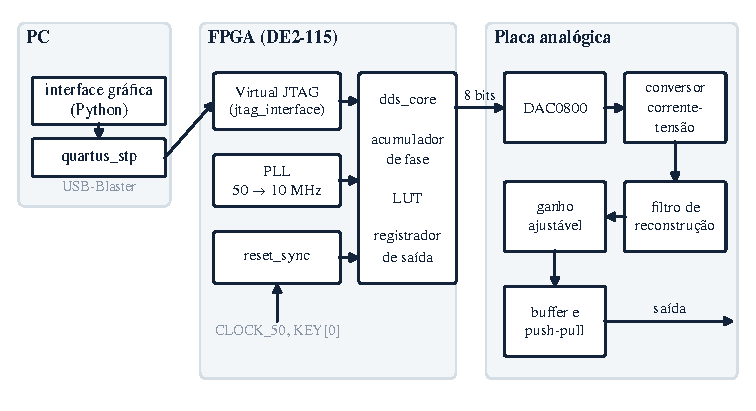
\includegraphics[width=\textwidth]{./figuras/sistema}
	\legend{Fonte~---~Autoria própria.}
\end{figure}

\section{Especificações}

A Tabela~\ref{tab:especificacoes} reúne os parâmetros do gerador. A frequência de clock de 10~MHz foi escolhida pelo tempo de acomodação típico do DAC0800, de 100~ns \cite{ti2013}: com um clock mais rápido, as amostras mudariam antes de o conversor se acomodar. O acumulador de 32~bits dá a resolução de 2,33~mHz da Equação~(\ref{eq:resolucao}). A tabela de 1024~amostras (\(P = 10\)) limita os espúrios de truncamento a cerca de \(-60\)~dBc, valor próximo ao limite de cerca de 50~dB imposto pela quantização em 8~bits, conforme as Equações~(\ref{eq:snr}) e (\ref{eq:sfdr}).

A frequência é pedida pelo computador como um inteiro em hertz, de 18~bits, que é a largura do registrador de dados do protocolo (Seção~\ref{sec:controle}). A frequência máxima, de 262\,143~Hz, fica muito abaixo do limite de Nyquist de 5~MHz e garante pelo menos 38 amostras por período.

\begin{table}
	\caption{Especificações do gerador.}
	\label{tab:especificacoes}
	\begin{tabular}{l l}\toprule
		Parâmetro & Valor\\\midrule
		Clock do \ac{dds} (\(f_{clk}\)) & 10~MHz, gerado por \ac{pll} a partir de 50~MHz\\
		Acumulador de fase (\(N\)) & 32~bits\\
		Resolução de frequência (\(\Delta f\)) & 2,33~mHz\\
		Endereço da tabela (\(P\)) & 10~bits (1024 amostras por período)\\
		Amostra e \ac{dac} (\(D\)) & 8~bits, binário deslocado (zero em 128)\\
		Faixa de frequência & 0 a 262\,143~Hz, inteiro em hertz\\
		Formas de onda & seno, rampa, sinc e arbitrária\\
		Forma inicial da tabela arbitrária & eletrocardiograma sintético\\
		Configuração após o \eng{reset} & seno de 1~kHz\\
		Controle & computador, via Virtual \ac{jtag} e USB-Blaster\\\bottomrule
	\end{tabular}
	\legend{Fonte~---~Autoria própria.}
\end{table}

\section{Ponto de partida: o código legado}\label{sec:legado}

O projeto partiu de uma versão anterior do gerador, usada em bancada até setembro de 2026 e guardada no repositório em \cod{fpga/legado/}. Essa versão segue a arquitetura clássica da Figura~\ref{fig:dds_blocos}: um acumulador de fase de 32~bits e uma tabela de seno de 256 posições de 8~bits, endereçada pelos 8~bits mais significativos da fase. Todo o circuito roda no oscilador de 50~MHz da placa. Um contador gera um pulso de habilitação a cada 50 ciclos, de modo que o acumulador avança e o \ac{dac} recebe uma amostra nova a 1~MHz. A palavra de sintonia vem de cinco constantes calculadas à mão e escolhidas pelas chaves SW0 a SW4 da placa: 100~Hz, 1~kHz, 10~kHz, 100~kHz e 300~kHz. A amostra passa por um registrador antes dos pinos, e o pino 2 do conector de expansão leva um clock de 1~MHz para um \ac{dac} com registrador de entrada.

Essa versão comprovou a cadeia completa, do \ac{fpga} à placa analógica, mas suas limitações orientaram o projeto final (Tabela~\ref{tab:legado}). Ela só gerava senos, em cinco frequências fixas, e qualquer outra frequência exigia recalcular a constante e recompilar o projeto. Com a taxa de 1~MHz, a 300~kHz restavam pouco mais de três amostras por período, e a tabela de 256 posições limita o maior espúrio de truncamento de fase a cerca de \(-48\)~dBc, pela Equação~(\ref{eq:sfdr}). O código tinha três entidades, com o divisor, a seleção de frequência e o registrador de saída reunidos no topo, e foi verificado apenas por inspeção visual das formas de onda no simulador. Do código legado, o projeto final manteve a pinagem do \ac{dac}, para que a placa analógica e o cabo continuassem os mesmos, e o registrador de saída.

\begin{table}
	\caption{Comparação entre o código legado e o projeto final.}
	\label{tab:legado}
	\begin{tabular}{p{0.2\textwidth} p{0.36\textwidth} p{0.36\textwidth}}\toprule
		& Código legado & Projeto final\\\midrule
		Taxa de amostras & 1~MHz, habilitação a cada 50 ciclos de 50~MHz & 10~MHz, gerada por um \ac{pll}\\
		Tabelas & seno, \(256 \times 8\)~bits & seno, rampa, sinc e arbitrária regravável, \(1024 \times 8\)~bits\\
		Frequência & cinco valores fixos, de 100~Hz a 300~kHz & qualquer inteiro de 0 a 262\,143~Hz\\
		Palavra de sintonia & constantes calculadas à mão & multiplicação em ponto fixo no \ac{fpga}\\
		Controle & chaves da placa & computador, pelo Virtual \ac{jtag}\\
		Organização & três entidades & uma entidade por função\\
		Verificação & inspeção visual no simulador & 16 \eng{testbenches} auto-verificáveis\\
		Recursos & 72 elementos lógicos e 2\,048 bits de memória & 378 elementos lógicos e 32\,768 bits de memória\\\bottomrule
	\end{tabular}
	\legend{Fonte~---~Autoria própria.}
\end{table}

\section{Projeto do núcleo digital}

\subsection{Organização hierárquica}

O projeto digital foi organizado em blocos encapsulados: cada função fica em uma entidade \ac{vhdl} própria, com portas bem definidas, e as entidades de nível mais alto apenas instanciam e ligam as de nível mais baixo. A entidade do topo, \cod{DDS}, não contém lógica: liga o \ac{pll}, o sincronizador de \eng{reset}, o controle pelo computador, o núcleo \ac{dds} e a saída de clock do \ac{dac} aos pinos da placa. A Figura~\ref{fig:hierarquia} mostra a hierarquia completa.

As constantes compartilhadas, como as larguras do caminho de dados, os códigos das instruções do protocolo e os códigos das formas de onda, ficam em um único pacote, \cod{dds\_pkg}. Assim, cada valor é definido em um único lugar, e os blocos e os \eng{testbenches} usam as mesmas definições.

\begin{figure}
	\caption{Hierarquia das entidades \acs{vhdl} do projeto. Os blocos em cinza são \acsp{ip} gerados pelas ferramentas da Intel.}
	\label{fig:hierarquia}
	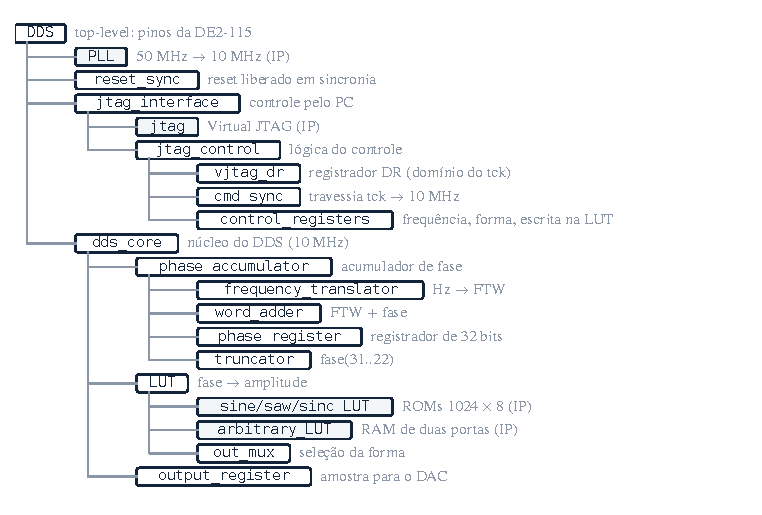
\includegraphics[width=\textwidth]{./figuras/hierarquia}
	\legend{Fonte~---~Autoria própria.}
\end{figure}

\subsection{Acumulador de fase e conversão de frequência}

O acumulador de fase (\cod{phase\_accumulator}) é composto por quatro blocos: o conversor de frequência (\cod{frequency\_translator}), o somador de 32~bits (\cod{word\_adder}), o registrador de fase (\cod{phase\_register}), que atualiza na borda de subida do clock e tem \eng{reset} assíncrono, e o truncador (\cod{truncator}), que entrega os 10~bits mais significativos da fase como endereço da tabela.

Pela Equação~(\ref{eq:fout}), a palavra de sintonia para uma frequência \(f\) é \(M = f \cdot 2^{32}/f_{clk}\), o que exigiria uma divisão. Como \(f_{clk}\) é fixo, a divisão foi substituída por uma multiplicação por uma constante em ponto fixo, com 24~bits fracionários:
\begin{equation}\label{eq:ftw}
	K = \operatorname{round}\!\left(\frac{2^{56}}{f_{clk}}\right) = 7\,205\,759\,404, \qquad M = \left\lfloor \frac{f \cdot K}{2^{24}} \right\rfloor.
\end{equation}
O produto de \(f\) (18~bits) por \(K\) (33~bits) tem 51~bits, e o deslocamento de 24~bits para a direita é apenas a escolha dos fios de saída. Como \(K\) é ligeiramente maior que o valor exato, o erro de \(M\) fica abaixo de 1~\ac{lsb} para toda a faixa de entrada, o que corresponde a um erro de frequência menor que \(\Delta f\). Na síntese, a multiplicação ocupa quatro multiplicadores de \(9 \times 9\)~bits do \ac{fpga}.

\subsection{Tabelas de forma de onda}

A conversão de fase em amplitude (\cod{LUT}) reúne quatro memórias de \(1024 \times 8\)~bits, implementadas pelo \ac{ip} \cod{altsyncram} nos blocos M9K, e um multiplexador (\cod{out\_mux}) controlado pelo sinal \cod{sel}. Três delas são \acp{rom} inicializadas por arquivos \ac{mif}, gerados conforme a Equação~(\ref{eq:lut_seno}):
\begin{itemize}
	\item seno (\cod{sel} = \cod{00}): \(\operatorname{round}(128 + 127\sin(2\pi n/1024))\);
	\item rampa (\cod{sel} = \cod{01}): subida e descida linear, em fase com o seno;
	\item sinc (\cod{sel} = \cod{10}): \(\operatorname{round}(128 + 127\,\mathrm{sinc}((n-512)/64))\), com o argumento entre \(-8\) e 8.
\end{itemize}

A quarta memória (\cod{sel} = \cod{11}) é uma \ac{ram} de duas portas, que guarda a forma arbitrária. A porta de leitura é endereçada pela fase, como as \acp{rom}; a porta de escrita é endereçada pelo computador. Com portas separadas, a tabela pode ser reescrita sem interromper a leitura. Na configuração do \ac{fpga}, a \ac{ram} recebe um eletrocardiograma sintético, gerado com o modelo dinâmico ECGSYN \cites{mcsharry2003,goldberger2000}: três equações diferenciais acopladas, com as ondas P, Q, R, S e T representadas por gaussianas na fase, e intervalos entre batimentos estocásticos, com espectro bimodal. Foram usados 120 batimentos por minuto em média, desvio de 3 batimentos por minuto e ruído de medida de 0,015~mV. A tabela contém dois batimentos, recortados no segmento TP para emendar sem descontinuidade; assim, com \(f = 1\)~Hz, a saída é um \ac{ecg} de 120 batimentos por minuto. A Figura~\ref{fig:luts} mostra o conteúdo das quatro tabelas.

\begin{figure}
	\caption{Conteúdo das quatro tabelas de forma de onda.}
	\label{fig:luts}
	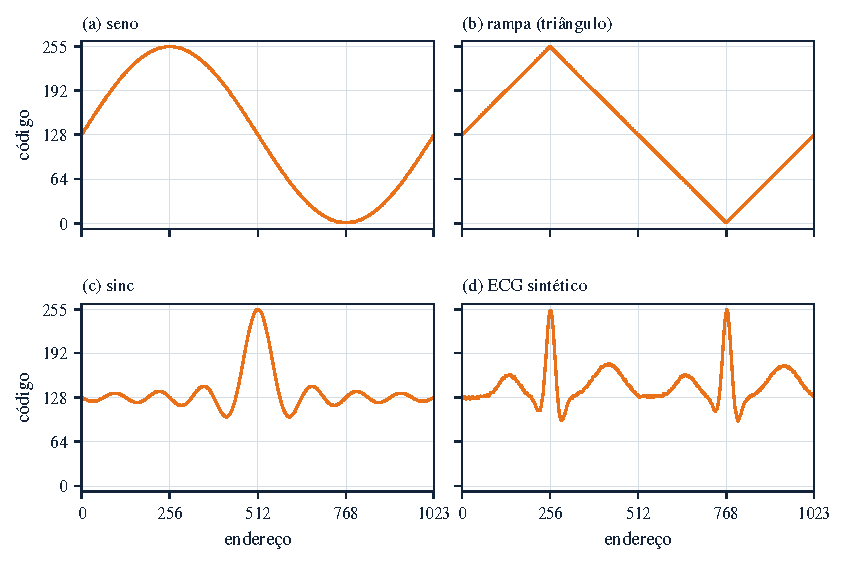
\includegraphics[width=\textwidth]{./figuras/luts}
	\legend{Fonte~---~Autoria própria.}
\end{figure}

As memórias registram o endereço e a saída, de modo que a amostra sai dois clocks depois do endereço. Após o multiplexador, a amostra passa por um registrador de saída (\cod{output\_register}), que no \eng{reset} assume o código 128, o zero do sinal. Esse registrador foi colocado nos registradores de entrada e saída do \ac{fpga}, junto aos pinos, para que os 8~bits mudem na mesma borda. Isso é importante porque o DAC0800 não tem registrador de entrada: bits que mudassem em instantes diferentes produziriam códigos intermediários na saída. O núcleo \cod{dds\_core} reúne o acumulador de fase, as tabelas e o registrador de saída; da fase até o pino do \ac{dac}, a latência é de três clocks.

\subsection{Controle pelo computador}\label{sec:controle}

O protocolo usa um registrador de instrução virtual de 2~bits e um registrador de dados de 18~bits, deslocado com o \ac{lsb} primeiro, conforme a Tabela~\ref{tab:protocolo}.

\begin{table}
	\caption{Instruções do protocolo de controle.}
	\label{tab:protocolo}
	\begin{tabular}{c l l}\toprule
		IR & Instrução & Conteúdo do DR (18~bits)\\\midrule
		\cod{00} & nenhuma (\eng{bypass}) & ---\\
		\cod{01} & frequência & frequência em hertz\\
		\cod{10} & forma de onda & \cod{sel} nos 2~bits menos significativos\\
		\cod{11} & escrita na tabela arbitrária & endereço (bits 17 a 8) e dado (bits 7 a 0)\\\bottomrule
	\end{tabular}
	\legend{Fonte~---~Autoria própria.}
\end{table}

O controle foi dividido em três blocos, um para cada domínio de clock e para a travessia entre eles:
\begin{description}
	\item[\cod{vjtag\_dr}] --- no domínio do \cod{tck}, desloca o registrador de dados durante o Shift-DR. No Update-DR, guarda a instrução e o valor deslocado e inverte o nível do sinal \cod{cmd\_toggle}, avisando que há um comando novo. No Capture-DR, carrega no registrador o último valor escrito com a mesma instrução, o que permite ler a configuração pelo \ac{jtag} para depuração. Na instrução \cod{00}, a saída \cod{tdo} vem de um registrador de \eng{bypass} de 1~bit;
	\item[\cod{cmd\_sync}] --- passa o comando para o domínio de 10~MHz pela técnica do \eng{toggle} descrita na Seção~\ref{sec:cdc}: apenas \cod{cmd\_toggle} passa por um sincronizador de três \eng{flip-flops}; quando sua mudança é detectada, os 20~bits do comando já estão estáveis e são copiados, com um pulso de um clock em \cod{dst\_valid}. A técnica exige que dois comandos estejam separados por mais de quatro ciclos de 10~MHz (0,4~\(\mu\)s). Um deslocamento de 18~bits leva mais de 22 ciclos de \cod{tck}, ou 3,7~\(\mu\)s a 6~MHz, frequência máxima do USB-Blaster, de forma que o requisito é sempre atendido;
	\item[\cod{control\_registers}] --- no domínio de 10~MHz, decodifica cada comando e atualiza os registradores de frequência e de forma de onda, ou gera um pulso de um clock na porta de escrita da \ac{ram}. Após o \eng{reset}, os registradores assumem 1~kHz e seno, de modo que a placa gera um sinal sem depender do computador.
\end{description}

Os três blocos foram agrupados na entidade \cod{jtag\_control}, que contém toda a lógica do controle mas não o \ac{ip} do Virtual \ac{jtag}. O \ac{ip} e o \cod{jtag\_control} são instanciados juntos em \cod{jtag\_interface}. Essa separação permite simular o controle completo, com o \eng{testbench} fazendo o papel do \ac{ip}, cujo modelo de simulação não gera sinais.

\subsection{Clock, reset e pinagem}

O \ac{pll} gera o clock de 10~MHz dividindo por cinco o oscilador de 50~MHz. O \eng{reset} do sistema vem do botão KEY[0] e da indicação de travamento do \ac{pll}, e passa por um sincronizador (\cod{reset\_sync}): entra em \eng{reset} de forma assíncrona, assim que o botão é pressionado, e sai em sincronia com o clock, três bordas depois de o botão ser solto. Assim, todos os registradores saem do \eng{reset} na mesma borda.

A Tabela~\ref{tab:pinos} mostra a pinagem, a mesma do código legado (Seção~\ref{sec:legado}), e a Figura~\ref{fig:pin_planner} mostra essas atribuições no Pin Planner do Quartus. O barramento do \ac{dac} usa os pinos 3 a 10 do conector de expansão, e o pino 1 é mantido em nível baixo como referência de terra no cabo. O pino 2 leva o clock de 10~MHz invertido, gerado pela entidade \cod{dac\_clock} com um registrador de saída de taxa dupla (\cod{altddio\_out}), o que evita passar o clock pela lógica. A borda de subida desse clock ocorre 50~ns depois da mudança dos bits, no meio da amostra. O DAC0800 não usa clock, mas o pino permite ligar um \ac{dac} com registrador de entrada e serve de gatilho para o osciloscópio. Dois \eng{LEDs} indicam o travamento do \ac{pll} e a chegada de cada comando do computador. A Tabela~\ref{tab:barramento} mostra o caminho de cada bit até o \acs{dac}: do pino do \acs{fpga} ao conector de expansão JP5 da DE2-115, dele ao conector J1 da placa analógica e, por fim, ao pino do DAC0800. A Figura~\ref{fig:jp5} mostra a disposição do JP5: os pinos ímpares ficam em uma fileira e os pares na outra, e o pino \(n\) corresponde ao GPIO[\(n - 1\)]. O fabricante numera as entradas do DAC0800 do bit mais significativo para o menos significativo, de B1 a B8, e por isso o bit 0 do \acs{fpga} chega à entrada B8, e o bit 7, à B1.

\begin{table}
	\caption{Pinagem do \acs{fpga} na placa DE2-115.}
	\label{tab:pinos}
	\begin{tabular}{l l l l}\toprule
		Porta & Pino do \acs{fpga} & Sinal na placa & Padrão de E/S e corrente\\\midrule
		\cod{clk\_50} & PIN\_Y2 & CLOCK\_50 & LVTTL 3,3~V\\
		\cod{rst\_n} & PIN\_M23 & botão KEY[0] & LVTTL 3,3~V\\
		\cod{dac(0)} & PIN\_AB21 & GPIO[2] & LVTTL 3,3~V, 8~mA\\
		\cod{dac(1)} & PIN\_Y17 & GPIO[3] & LVTTL 3,3~V, 8~mA\\
		\cod{dac(2)} & PIN\_AC21 & GPIO[4] & LVTTL 3,3~V, 8~mA\\
		\cod{dac(3)} & PIN\_Y16 & GPIO[5] & LVTTL 3,3~V, 8~mA\\
		\cod{dac(4)} & PIN\_AD21 & GPIO[6] & LVTTL 3,3~V, 8~mA\\
		\cod{dac(5)} & PIN\_AE16 & GPIO[7] & LVTTL 3,3~V, 8~mA\\
		\cod{dac(6)} & PIN\_AD15 & GPIO[8] & LVTTL 3,3~V, 8~mA\\
		\cod{dac(7)} & PIN\_AE15 & GPIO[9] & LVTTL 3,3~V, 8~mA\\
		\cod{dac\_clk} & PIN\_AC15 & GPIO[1] & LVTTL 3,3~V, 8~mA\\
		\cod{dac\_gnd} & PIN\_AB22 & GPIO[0] & LVTTL 3,3~V, 8~mA\\
		\cod{led\_locked} & PIN\_E21 & \eng{LED} LEDG[0] & 2,5~V, 8~mA\\
		\cod{led\_cmd} & PIN\_E22 & \eng{LED} LEDG[1] & 2,5~V, 8~mA\\\bottomrule
	\end{tabular}
	\legend{Fonte~---~Autoria própria.}
\end{table}

\begin{table}
	\caption{Ligação do barramento, do \acs{fpga} ao DAC0800.}
	\label{tab:barramento}
	\begin{tabular}{l l l c c c}\toprule
		Bit & Porta & Pino do \acs{fpga} & Conector JP5 & Conector J1 & Pino do DAC0800\\\midrule
		0 (\acs{lsb}) & \cod{dac(0)} & PIN\_AB21 & 3 & 1 & 12 (B8)\\
		1 & \cod{dac(1)} & PIN\_Y17 & 4 & 2 & 11 (B7)\\
		2 & \cod{dac(2)} & PIN\_AC21 & 5 & 3 & 10 (B6)\\
		3 & \cod{dac(3)} & PIN\_Y16 & 6 & 4 & 9 (B5)\\
		4 & \cod{dac(4)} & PIN\_AD21 & 7 & 5 & 8 (B4)\\
		5 & \cod{dac(5)} & PIN\_AE16 & 8 & 6 & 7 (B3)\\
		6 & \cod{dac(6)} & PIN\_AD15 & 9 & 7 & 6 (B2)\\
		7 (\acs{msb}) & \cod{dac(7)} & PIN\_AE15 & 10 & 8 & 5 (B1)\\
		--- & \cod{dac\_clk} & PIN\_AC15 & 2 & --- & ---\\
		--- & \cod{dac\_gnd} & PIN\_AB22 & 1 & --- & ---\\\bottomrule
	\end{tabular}
	\legend{Fonte~---~Autoria própria.}
\end{table}

\begin{figure}
	\caption{Atribuição dos pinos no Pin Planner do Quartus.}
	\label{fig:pin_planner}
	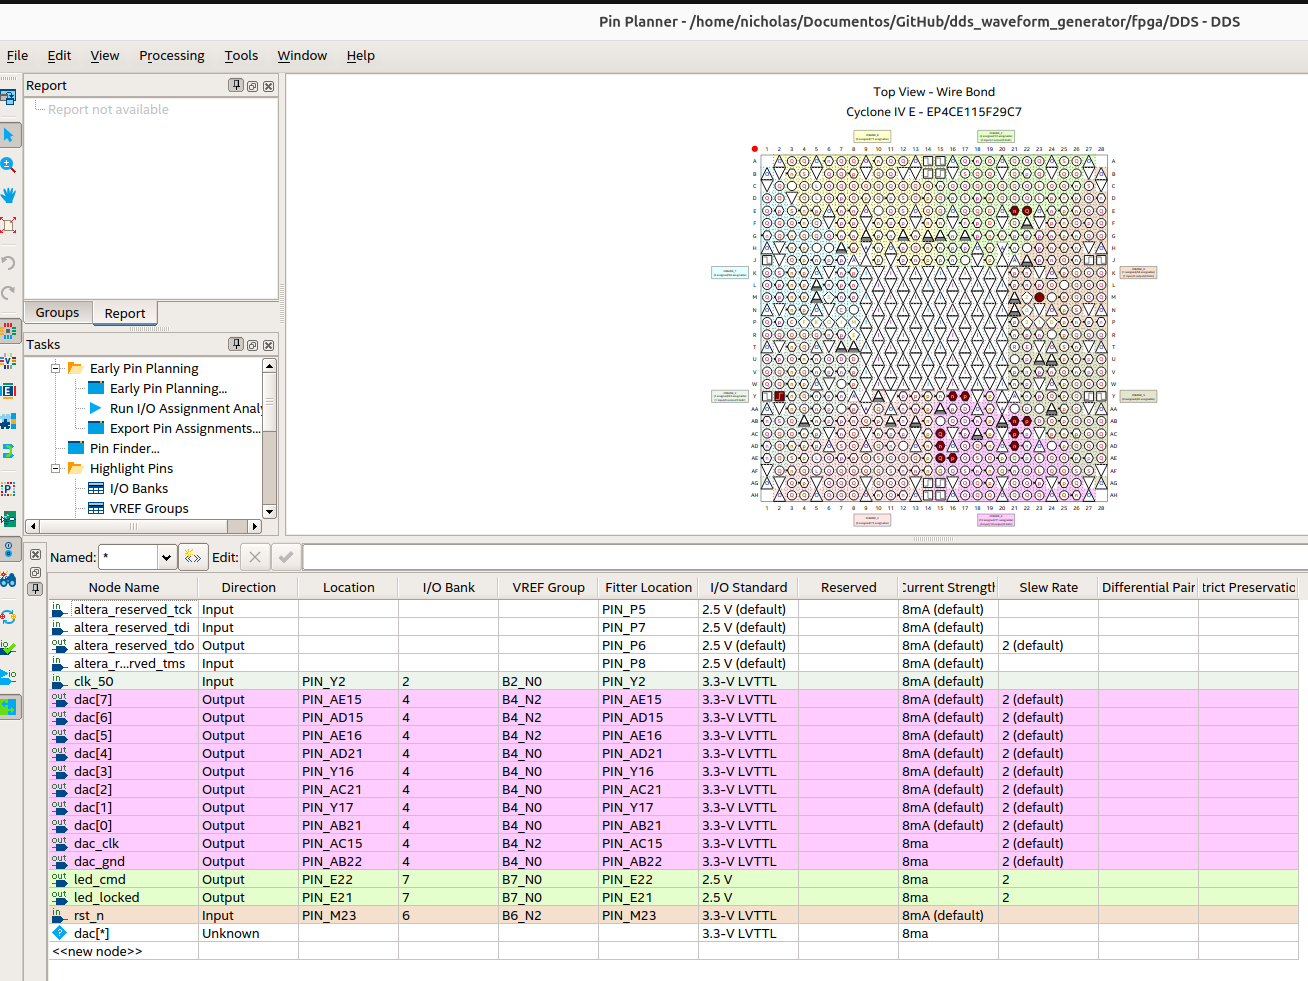
\includegraphics[width=\textwidth]{./figuras/pin_planner}
	\legend{Fonte~---~Autoria própria.}
\end{figure}

\begin{figure}
	\caption{Conector de expansão JP5 da DE2-115, com o pino do \acs{fpga} ligado a cada posição.}
	\label{fig:jp5}
	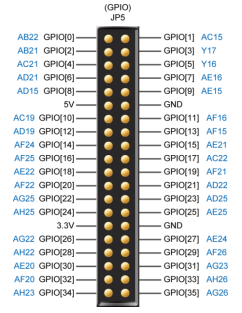
\includegraphics[width=0.4\textwidth]{./figuras/jp5_gpio}
	\legend{Fonte~---~Terasic Technologies \cite{terasic2010}.}
\end{figure}


As restrições de tempo foram descritas em um arquivo \ac{sdc}: o clock de 50~MHz e os clocks derivados do \ac{pll}; o clock do \ac{jtag} como assíncrono em relação aos demais, já que a travessia é tratada pelo \cod{cmd\_sync}; e caminhos sem requisito de tempo para o botão, os \eng{LEDs}, o barramento do \ac{dac}, que não usa clock, e o próprio clock do \ac{dac}, cuja relação com os dados é fixada pelos registradores junto aos pinos.

\section{Verificação por simulação}

Cada bloco do projeto digital tem um \eng{testbench} auto-verificável, escrito em \ac{vhdl}-2008 e executado no simulador GHDL \cite{ghdl2025}. Os blocos gerados pela Intel são simulados com os modelos da biblioteca \cod{altera\_mf}, distribuída com o Quartus. Cada \eng{testbench} compara a saída do bloco, ciclo a ciclo, com um modelo de referência escrito no próprio \eng{testbench}, conta os erros e termina com a mensagem \enquote{OK} apenas se não houver nenhum. Para o núcleo \ac{dds}, por exemplo, o modelo calcula a fase pela Equação~(\ref{eq:acumulador}), o endereço pelo truncamento e a amostra esperada pela tabela correspondente, considerando a latência de três clocks.

Os blocos do controle são verificados com um modelo de comportamento do Virtual \ac{jtag}: procedimentos que geram o \cod{tck}, a instrução e a sequência Capture-DR, Shift-DR e Update-DR, como o \ac{ip} faria a cada comando do \cod{quartus\_stp}. A Tabela~\ref{tab:testbenches} lista os 16 \eng{testbenches} e o que cada um confere. Um \eng{script} compila os fontes e executa todos eles em sequência. Para as figuras deste texto, os \eng{testbenches} são executados gravando os sinais de interesse em arquivos \ac{vcd}, que um \eng{script} em Python lê e desenha.

\begin{table}
	\caption{\eng{Testbenches} do projeto digital.}
	\label{tab:testbenches}
	\begin{tabular}{l p{0.62\textwidth}}\toprule
		\eng{Testbench} & O que é conferido\\\midrule
		\cod{tb\_frequency\_translator} & as \(2^{18}\) entradas: \ac{ftw} conforme a Equação~(\ref{eq:ftw}) e erro menor que 1~\ac{lsb}\\
		\cod{tb\_word\_adder} & soma com estouro, casos de borda e 10\,000 pares aleatórios\\
		\cod{tb\_phase\_register} & carga apenas na borda de subida e \eng{reset} assíncrono\\
		\cod{tb\_truncator} & endereço igual aos 10~bits mais significativos da fase\\
		\cod{tb\_phase\_accumulator} & endereço ciclo a ciclo, trocas de frequência sem salto de fase\\
		\cod{tb\_out\_mux} & seleção para cada código de \cod{sel}\\
		\cod{tb\_LUT} & os 1024 endereços das três \acp{rom} e da \ac{ram}, escrita durante a leitura\\
		\cod{tb\_output\_register} & código 128 no \eng{reset} e carga na borda\\
		\cod{tb\_dds\_core} & cada amostra contra o modelo, nas quatro formas e com trocas em operação\\
		\cod{tb\_reset\_sync} & entrada imediata e saída na terceira borda\\
		\cod{tb\_vjtag\_dr} & deslocamento, comando no Update-DR, leitura no Capture-DR e \eng{bypass}\\
		\cod{tb\_cmd\_sync} & 300 comandos de 6~MHz para 10~MHz, todos entregues uma vez e em ordem\\
		\cod{tb\_control\_registers} & valores após o \eng{reset}, decodificação e pulso de escrita\\
		\cod{tb\_jtag\_control} & do registrador de dados do \ac{jtag} até os registradores de configuração\\
		\cod{tb\_system} & do comando do computador até a amostra do \ac{dac}, incluindo o envio de uma tabela\\
		\cod{tb\_DDS} & entidade do topo com o \ac{pll}: clocks, \eng{LEDs}, seno de 1~kHz e \eng{reset}\\\bottomrule
	\end{tabular}
	\legend{Fonte~---~Autoria própria.}
\end{table}

\section{Interface com o usuário}

A interface gráfica foi escrita em Python 3.12, com a biblioteca Tkinter, e usa apenas a biblioteca padrão da linguagem. Ela mantém aberto um processo do \cod{quartus\_stp} e envia a ele comandos Tcl: trava o acesso ao \ac{jtag}, desloca a instrução uma vez e o registrador de dados uma vez para cada valor, e libera o acesso. Uma \eng{thread} separada executa os comandos em ordem e devolve os resultados por uma fila de eventos, de modo que a janela não trava durante o envio de uma tabela, que exige 1024 deslocamentos.

A interface permite escolher a frequência, mostrando a palavra de sintonia calculada pela Equação~(\ref{eq:ftw}), e a forma de onda; carregar a tabela arbitrária de um arquivo \ac{mif} ou de um arquivo de texto com 1024 valores, ou gerá-la a partir de formas prontas; visualizar a tabela antes do envio; e acompanhar as mensagens do \cod{quartus\_stp} em um console. A Figura~\ref{fig:interface} mostra a interface: no alto, a conexão \acs{jtag} e a carga da tabela arbitrária; à esquerda, a frequência, com a palavra de sintonia correspondente, a forma de onda e os parâmetros do sistema; ao centro, o gráfico da tabela arbitrária; e, abaixo, o console.

Para dispensar o terminal, a interface foi empacotada com o PyInstaller em um executável único, que já contém o Python, o Tkinter, o ícone e as tabelas \ac{mif}, e um atalho no menu de aplicativos a abre com dois cliques. Ela depende apenas do Quartus instalado, de onde vem o \cod{quartus\_stp}.

\begin{figure}
	\caption{Interface gráfica de controle do gerador.}
	\label{fig:interface}
	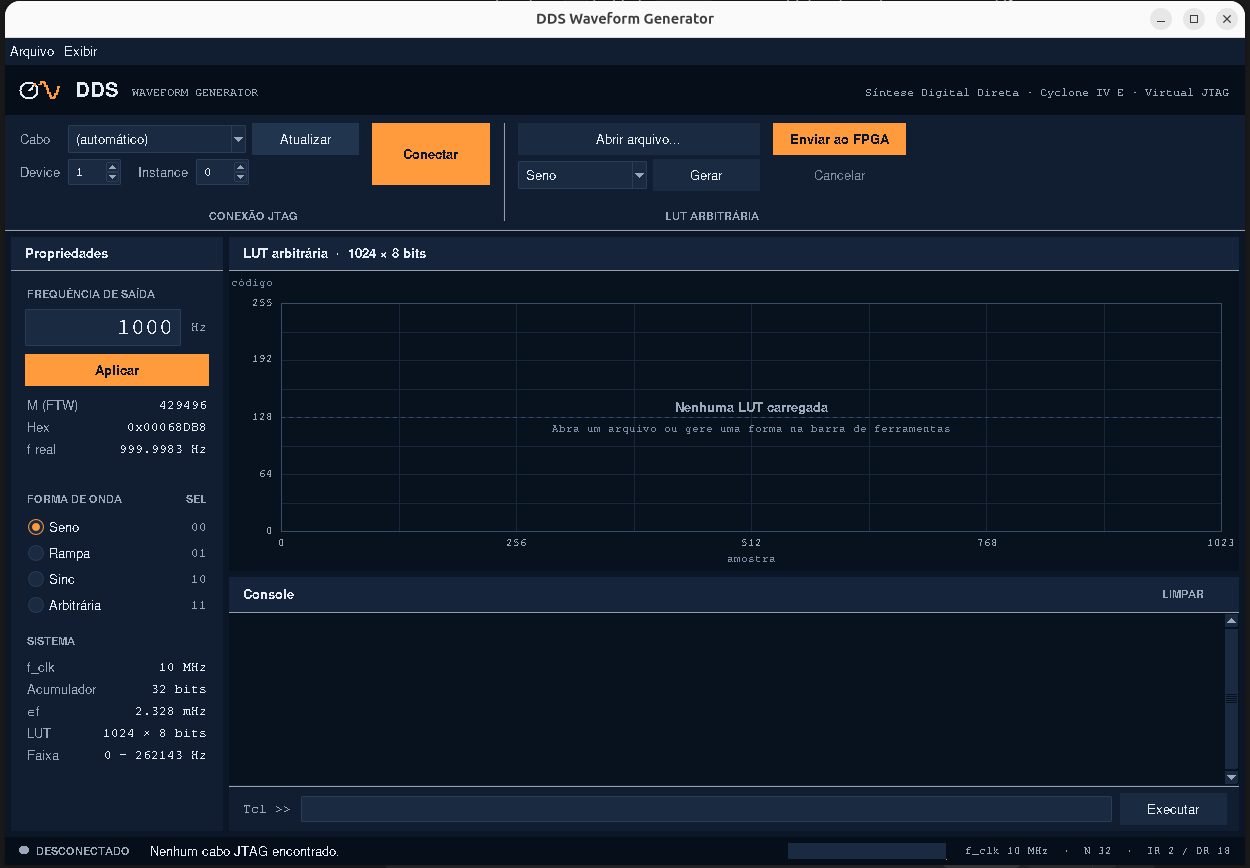
\includegraphics[width=\textwidth]{./figuras/interface}
	\legend{Fonte~---~Autoria própria.}
\end{figure}

\section{Placa analógica}

A placa analógica recebe os 8~bits pelo conector J1 e é alimentada com \(\pm15\)~V, para os amplificadores operacionais e o \ac{dac}, e +10~V, para a referência do \ac{dac}. O circuito tem cinco blocos, ligados conforme a Figura~\ref{fig:sistema}. Os valores a seguir são os da simulação do circuito, que segue a mesma topologia da placa.

O DAC0800 tem a referência de 10~V aplicada através de um resistor de 5~k\(\Omega\), o que, pela Equação~(\ref{eq:dac0800}), fixa \(I_{REF} = 2\)~mA e \(I_{FS} \approx 1{,}992\)~mA. Com o pino de limiar lógico no terra, o limiar das entradas é de 1,4~V, compatível com a lógica de 3,3~V do \ac{fpga}. Na placa, o pino DB7 do conector J1, que recebe o \ac{msb} da amostra, é ligado à entrada B1 do conversor, que é o seu \ac{msb}.

As duas saídas de corrente alimentam um amplificador de diferenças com quatro resistores de 1~k\(\Omega\), cuja saída é
\begin{equation}\label{eq:vdif}
	V_{dif} = \left(I_{OUT} - \overline{I_{OUT}}\right) \cdot 1~\mathrm{k}\Omega,
\end{equation}
que vai de \(-1{,}99\)~V, no código 0, a \(+1{,}99\)~V, no código 255. Em seguida, um filtro Sallen-Key de ganho unitário, com \(R_1 = R_2 = 48~\Omega\) e \(C_1 = C_2 = 3{,}3\)~nF, tem, pela Equação~(\ref{eq:sallen_key}), \(f_0 \approx 1{,}00\)~MHz e \(Q = 0{,}5\). A resposta em frequência, mostrada na Figura~\ref{fig:filtro}, tem atenuação de 3~dB em 647~kHz, perda de 0,6~dB na frequência máxima do gerador e atenuação de cerca de 40~dB em \(f_{clk}\), onde surgem as primeiras imagens.

\begin{figure}
	\caption{Resposta em frequência do filtro de reconstrução.}
	\label{fig:filtro}
	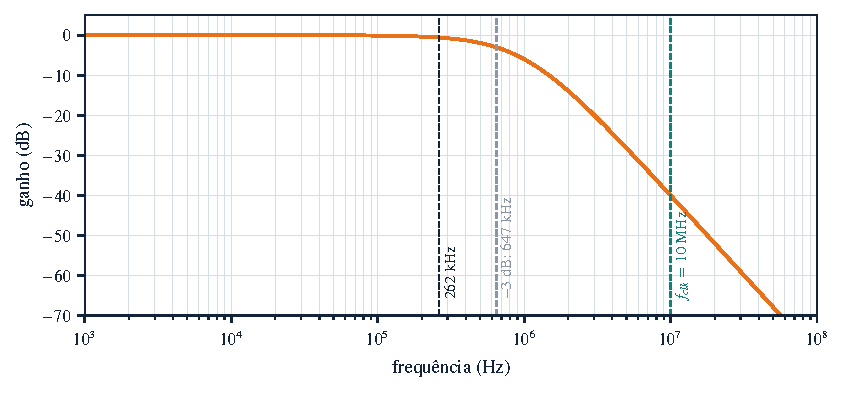
\includegraphics[width=\textwidth]{./figuras/filtro}
	\legend{Fonte~---~Autoria própria.}
\end{figure}

O ganho é ajustado por um amplificador inversor com um potenciômetro de 10~k\(\Omega\) (VR1). Por fim, um seguidor de tensão entrega o sinal ao conector de saída J7. Os quatro amplificadores são as quatro seções de um TL074.

A placa foi desenhada com mais um estágio depois do seguidor: um par complementar BC847 e BC857, polarizado por dois diodos LL4148 em classe AB, para aumentar a corrente de saída. Esse estágio foi retirado por apresentar distorção e resultados inesperados nos ensaios, e a saída passou a ser tomada diretamente do seguidor.

A placa foi projetada no Altium Designer e fabricada em duas faces. A Figura~\ref{fig:pcb_esquematico} mostra o esquemático, a Figura~\ref{fig:pcb_layout}, o layout das trilhas, e a Figura~\ref{fig:placa}, a vista tridimensional e a placa montada. O esquemático e o layout ainda incluem o estágio classe AB (Q1, Q2, D1, D2, R11 e R12), que foi retirado da montagem. O circuito, sem o estágio classe AB, foi simulado no LTspice com um macromodelo comportamental do DAC0800, escrito pelo autor a partir das características típicas da folha de dados \cite{ti2013,seifert2026spice} e descrito no Apêndice~\ref{ap:dac0800}: referência, divisão da corrente entre as saídas, limiar lógico, tempo de comutação de 70~ns e limites de conformidade das saídas. Os estímulos das entradas digitais são fontes lineares por partes geradas a partir da simulação do \ac{vhdl}, para uma senoide de 1~kHz. A Figura~\ref{fig:ltspice} mostra o esquemático simulado, com os nós cujas tensões são analisadas no Capítulo~\ref{cap:resultados}.

\begin{figure}
	\caption{Esquemático da simulação da placa analógica no LTspice: fontes dos estímulos (U7), DAC0800 (U1), conversor corrente-tensão (U2), estágio de ganho (U3), filtro de reconstrução (U4) e \eng{buffer} (U5).}
	\label{fig:ltspice}
	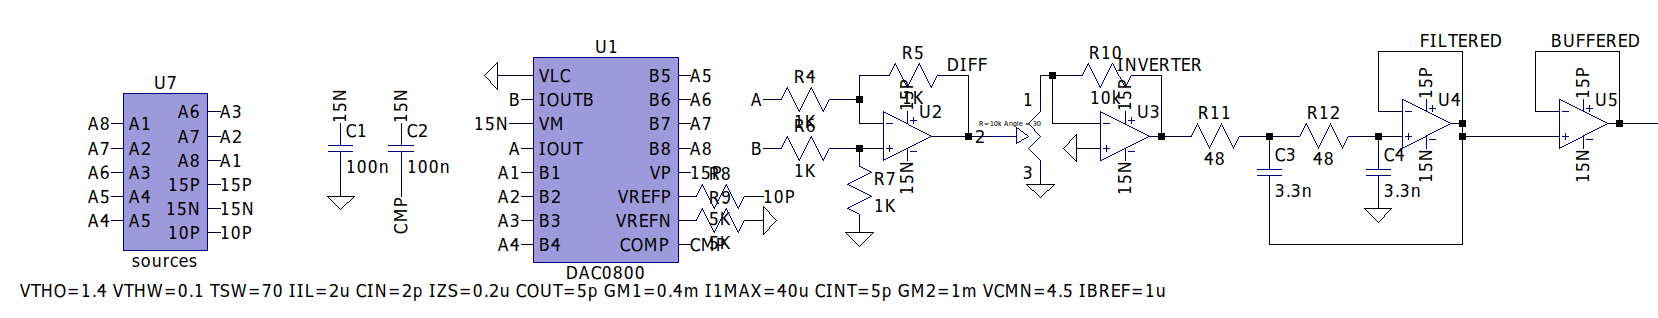
\includegraphics[width=\textwidth]{./figuras/ltspice_esquematico}
	\legend{Fonte~---~Autoria própria.}
\end{figure}


\begin{figure}
	\caption{Esquemático da placa analógica.}
	\label{fig:pcb_esquematico}
	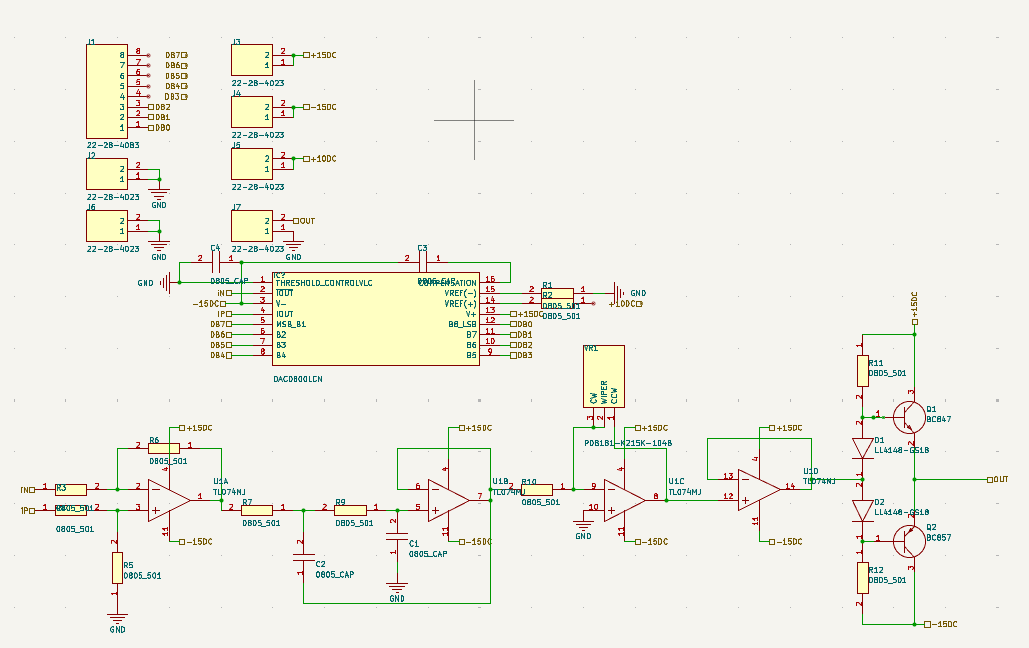
\includegraphics[width=\textwidth]{./figuras/pcb_esquematico}
	\legend{Fonte~---~Autoria própria.}
\end{figure}

\begin{figure}
	\caption{Layout da placa analógica: trilhas na face superior, em vermelho, e na inferior, em azul.}
	\label{fig:pcb_layout}
	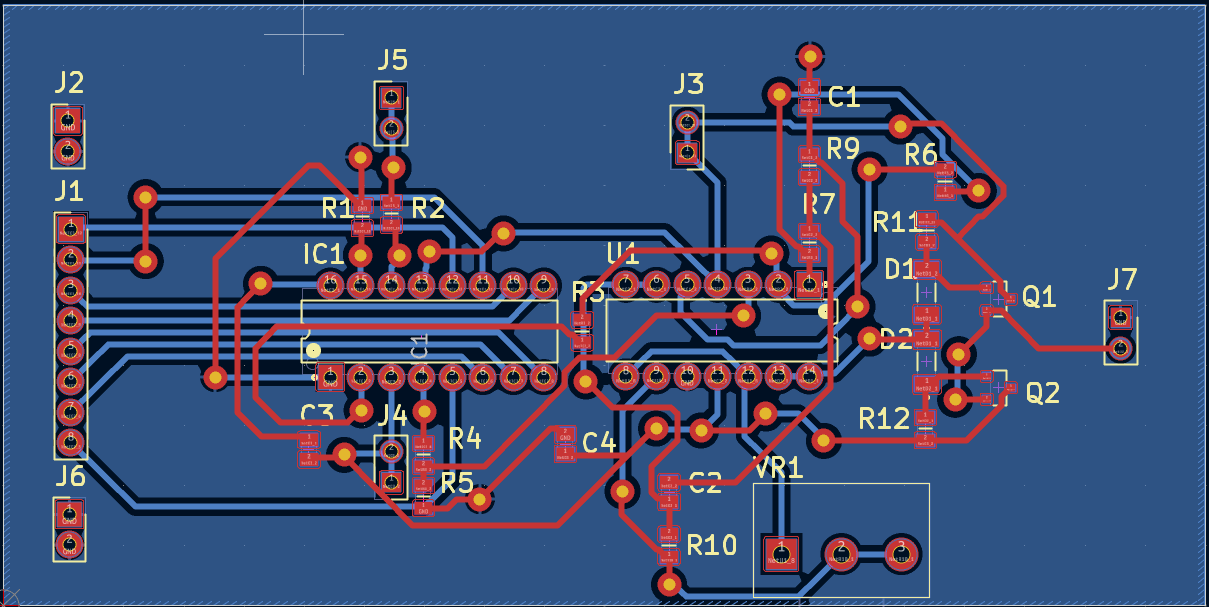
\includegraphics[width=\textwidth]{./figuras/pcb_layout}
	\legend{Fonte~---~Autoria própria.}
\end{figure}

\begin{figure}
	\caption{Placa analógica: (a) vista tridimensional; (b) placa montada, com o DAC0800 (IC1), o TL074 (U1) e o potenciômetro de ganho (VR1).}
	\label{fig:placa}
	\begin{minipage}[b]{0.6\textwidth}
		\centering
		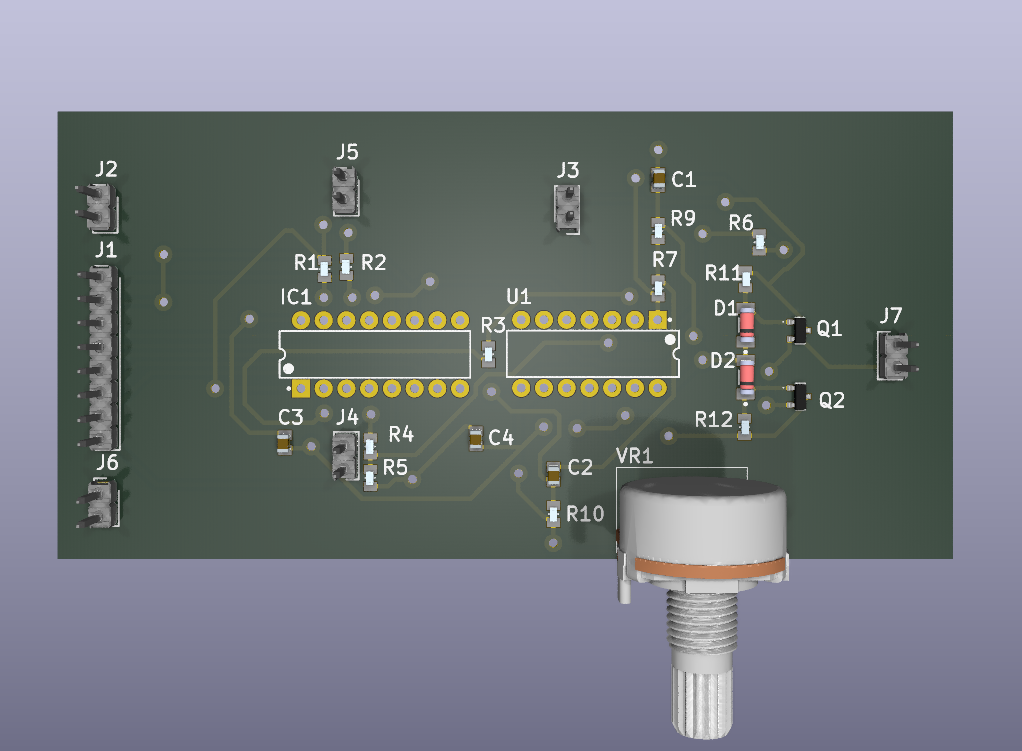
\includegraphics[height=6.4cm]{./figuras/pcb_3d}\\[2pt]
		{\smallfont (a)}
	\end{minipage}%
	\hfill
	\begin{minipage}[b]{0.36\textwidth}
		\centering
		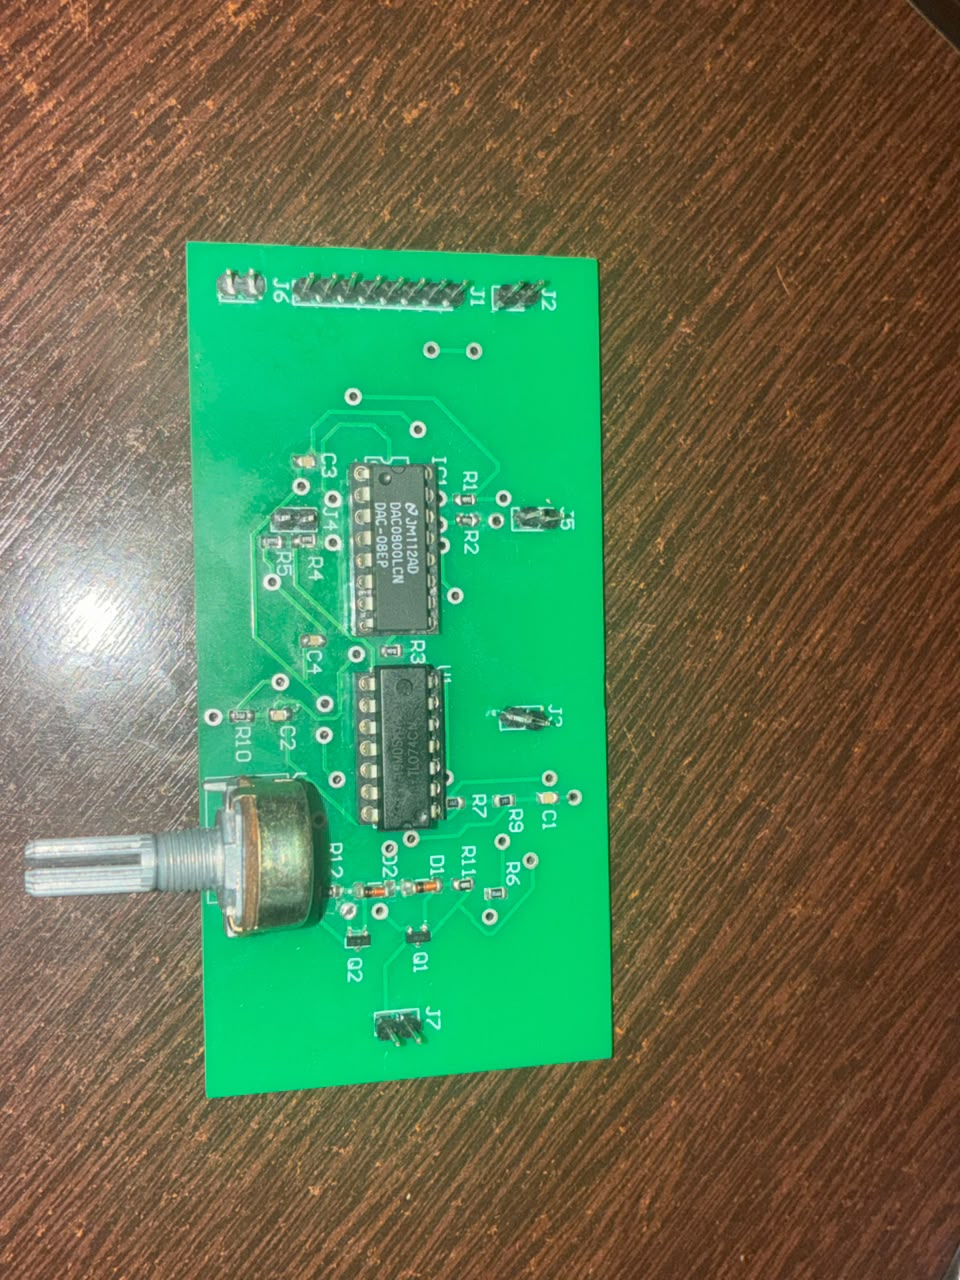
\includegraphics[height=6.4cm]{./figuras/placa}\\[2pt]
		{\smallfont (b)}
	\end{minipage}
	\legend{Fonte~---~Autoria própria.}
\end{figure}

\chapter{Resultados e discussões}\label{cap:resultados}

Este capítulo apresenta os resultados da síntese do projeto digital no \ac{fpga}, da verificação por simulação, da simulação da placa analógica e dos ensaios em bancada, discutindo cada um.

\section{Síntese e análise de tempo}

O projeto foi compilado no Quartus Prime 18.1 Lite para o EP4CE115F29C7. A Tabela~\ref{tab:recursos} mostra os recursos usados. O gerador ocupa menos de 1\% dos elementos lógicos do \ac{fpga}. Os 32\,768~bits de memória correspondem às quatro tabelas de \(1024 \times 8\)~bits, e os quatro multiplicadores de \(9 \times 9\)~bits são os da conversão de frequência da Equação~(\ref{eq:ftw}). Os registradores de saída do barramento do \ac{dac} foram efetivamente alocados nos registradores de entrada e saída, junto aos pinos.

\begin{table}
	\caption{Recursos do \acs{fpga} usados pelo projeto.}
	\label{tab:recursos}
	\begin{tabular}{l r r}\toprule
		Recurso & Usado & Disponível\\\midrule
		Elementos lógicos & 378 & 114\,480\\
		Registradores & 262 & ---\\
		Bits de memória & 32\,768 & 3\,981\,312\\
		Multiplicadores de \(9 \times 9\)~bits & 4 & 532\\
		\acp{pll} & 1 & 4\\
		Pinos & 13 & 529\\\bottomrule
	\end{tabular}
	\legend{Fonte~---~Autoria própria.}
\end{table}

A Tabela~\ref{tab:tempo} resume a análise de tempo, no modelo mais lento do dispositivo (1,2~V e 85~°C). O domínio de 10~MHz poderia operar a até 100,25~MHz, uma margem de dez vezes. O domínio do \ac{jtag} poderia operar a até 29,68~MHz, contra os 6~MHz máximos do USB-Blaster. Todas as folgas são positivas, e nenhum caminho ficou sem restrição de tempo.

\begin{table}
	\caption{Resultado da análise de tempo (modelo lento, 85~°C).}
	\label{tab:tempo}
	\begin{tabular}{l c c c}\toprule
		Domínio de clock & Frequência máxima & Folga de \eng{setup} & Folga de \eng{hold}\\\midrule
		10~MHz (\ac{pll}) & 100,25~MHz & 90,0~ns & 0,30~ns\\
		\cod{tck} (\ac{jtag}) & 29,68~MHz & 33,2~ns & 0,40~ns\\\bottomrule
	\end{tabular}
	\legend{Fonte~---~Autoria própria.}
\end{table}

A análise de metaestabilidade do Quartus identificou duas cadeias sincronizadoras de três registradores, a do \cod{cmd\_sync} e a do \cod{reset\_sync}, com tempo de acomodação disponível de pelo menos 294~ns, e estimou um tempo médio entre falhas típico superior a \(10^{9}\) anos para o projeto.

\section{Verificação do núcleo digital}

Os 16 \eng{testbenches} da Tabela~\ref{tab:testbenches} terminaram sem nenhum erro. A execução completa leva cerca de 2,5~min em um computador pessoal; os mais demorados são o \cod{tb\_frequency\_translator}, que percorre as \(2^{18}\) entradas, e o \cod{tb\_DDS}, que simula o modelo do \ac{pll}. As figuras de simulação desta seção e das seguintes foram desenhadas a partir dos sinais gravados nessas simulações. Antes de cada uma, uma figura mostra o bloco correspondente no RTL Viewer do Quartus, que desenha o circuito inferido a partir do \ac{vhdl}, depois da análise e elaboração do projeto. Os blocos menores, que não são discutidos aqui, têm a visão RTL e a simulação reunidas no Apêndice~\ref{ap:blocos}.

\subsection{Conversão de frequência}

No RTL, o conversor de frequência é um único multiplicador, \cod{Mult0}, entre a frequência de 18~bits e a constante \(K\) de 33~bits (\cod{33'h1ad7f29ac}), como mostra a Figura~\ref{fig:rtl_ftw}. Dos 51~bits do produto, os bits 50 a 24 formam a palavra de sintonia; o deslocamento da Equação~(\ref{eq:ftw}) não gera lógica.

\begin{figure}
	\caption{Visão RTL do conversor de frequência (\cod{frequency\_translator}).}
	\label{fig:rtl_ftw}
	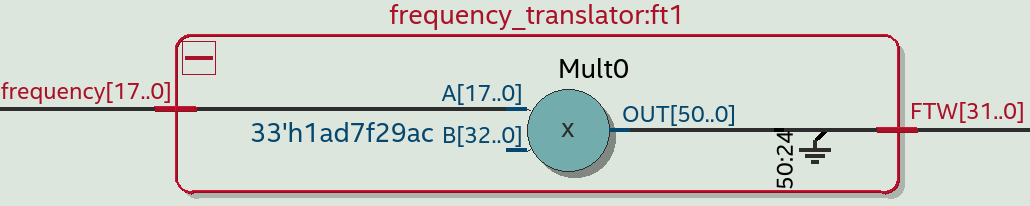
\includegraphics[width=\textwidth]{./figuras/rtl_frequency_translator}
	\legend{Fonte~---~Autoria própria.}
\end{figure}

A Figura~\ref{fig:tb_ftw}(a) mostra a palavra de sintonia para todas as entradas, e a Figura~\ref{fig:tb_ftw}(b) mostra o erro em relação ao valor exato \(f \cdot 2^{32}/f_{clk}\), no trecho de 0 a 2~kHz. O erro é sempre menor que 1~\ac{lsb}, como previsto no Capítulo~\ref{cap:metodologia}: o maior valor em toda a faixa é de 0,99986~\ac{lsb}, em 2\,752~Hz, o que corresponde a um erro de frequência de 2,328~mHz, menor que a resolução \(\Delta f\). O padrão em linhas inclinadas vem da parte fracionária de \(f \cdot 2^{32}/f_{clk}\), que avança 0,4967 a cada hertz.

\begin{figure}
	\caption{Conversão de frequência: (a) palavra de sintonia para as \(2^{18}\) entradas; (b) erro de truncamento.}
	\label{fig:tb_ftw}
	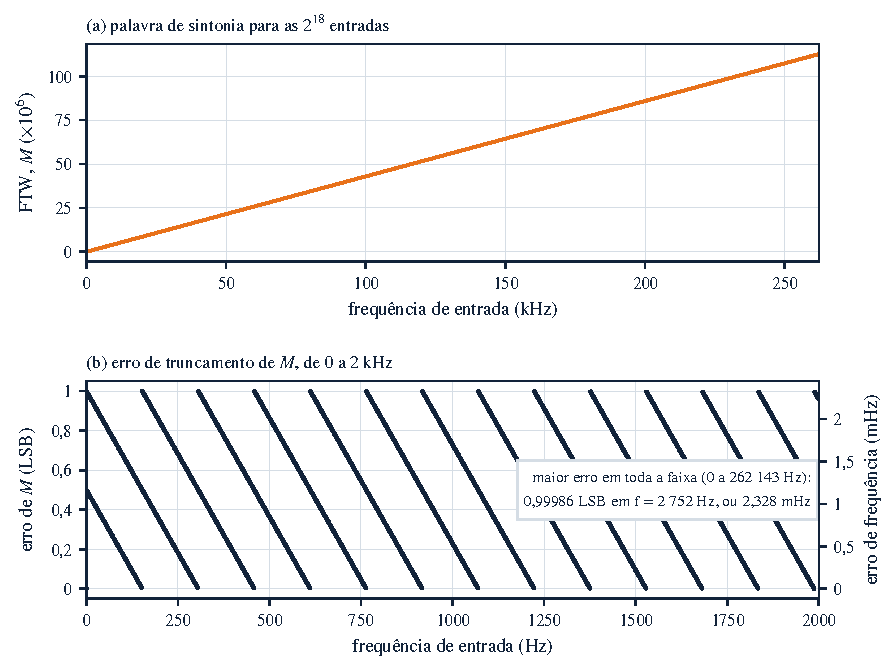
\includegraphics[width=\textwidth]{./figuras/tb_frequency_translator}
	\legend{Fonte~---~Autoria própria.}
\end{figure}

\subsection{Acumulador de fase}

A Figura~\ref{fig:rtl_acc} mostra o acumulador de fase no RTL: o conversor de frequência alimenta o somador, cuja saída é guardada no registrador de fase; a saída do registrador volta ao somador e segue para o truncador.

\begin{figure}
	\caption{Visão RTL do acumulador de fase (\cod{phase\_accumulator}).}
	\label{fig:rtl_acc}
	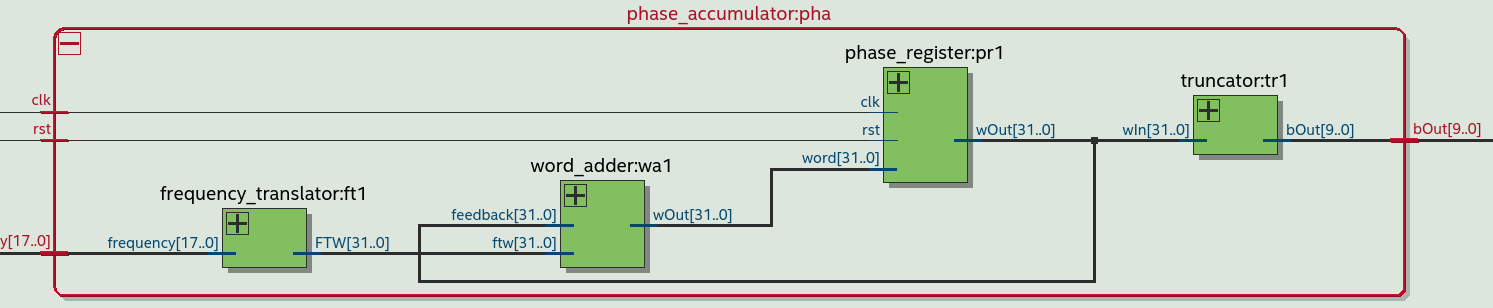
\includegraphics[width=\textwidth]{./figuras/rtl_phase_accumulator}
	\legend{Fonte~---~Autoria própria.}
\end{figure}

A Figura~\ref{fig:tb_acc} mostra o endereço da tabela durante a simulação do acumulador de fase. Em 1~kHz, a palavra de sintonia é 429\,496, e a frequência gerada é de 999,9983~Hz; o endereço percorre os 1024 valores em rampas de 1~ms, e três voltas se completam em 30\,001 clocks (Figura~\ref{fig:tb_acc}(a)). As Figuras~\ref{fig:tb_acc}(b) e (c) mostram as trocas de frequência com o acumulador em operação: em cada troca, o endereço continua do valor em que estava, sem salto, e passa a avançar no novo passo. Com 0~Hz, a fase permanece parada. Em todos os clocks, o endereço coincidiu com o do modelo de referência.

\begin{figure}
	\caption{Endereço da tabela no acumulador de fase: (a) em 1~kHz; (b) e (c) nas trocas de frequência.}
	\label{fig:tb_acc}
	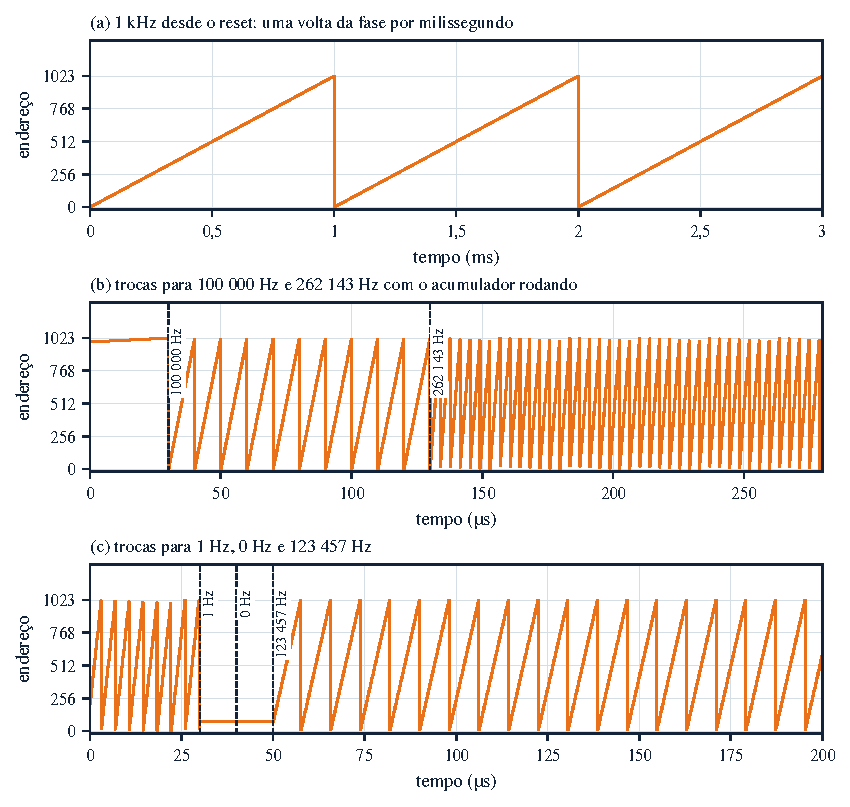
\includegraphics[width=\textwidth]{./figuras/tb_phase_accumulator}
	\legend{Fonte~---~Autoria própria.}
\end{figure}

\subsection{Tabelas de forma de onda}

A Figura~\ref{fig:rtl_lut} mostra a conversão de fase em amplitude no RTL: as três \acsp{rom} e a \acs{ram} recebem o mesmo endereço de leitura, a \acs{ram} tem também as entradas de escrita, e o multiplexador escolhe a saída pelo sinal \cod{sel}. As memórias aparecem como blocos fechados, pois são \acsp{ip}.

\begin{figure}
	\caption{Visão RTL das tabelas de forma de onda (\cod{LUT}).}
	\label{fig:rtl_lut}
	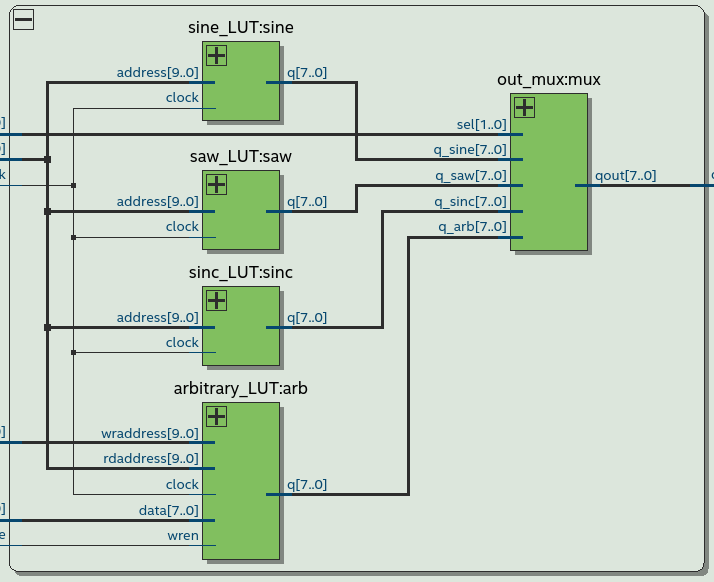
\includegraphics[width=0.75\textwidth]{./figuras/rtl_LUT}
	\legend{Fonte~---~Autoria própria.}
\end{figure}

A Figura~\ref{fig:tb_lut} mostra, para cada memória, o valor lido em cada um dos 1024 endereços, percorridos em ordem embaralhada, sobre o conteúdo esperado dos arquivos \ac{mif}. As seis varreduras terminaram sem nenhuma diferença. A varredura (e) foi feita com a escrita de um novo padrão em toda a \ac{ram} ao mesmo tempo, e confirma que a escrita não perturba a leitura das outras tabelas; a varredura (f) confirma que a \ac{ram} devolve o padrão escrito, três períodos de uma senoide. A Figura~\ref{fig:tb_lut_lat} mostra a latência de dois clocks entre o endereço e a amostra.

\begin{figure}
	\caption{Leitura das quatro memórias, endereço a endereço, comparada com o conteúdo esperado.}
	\label{fig:tb_lut}
	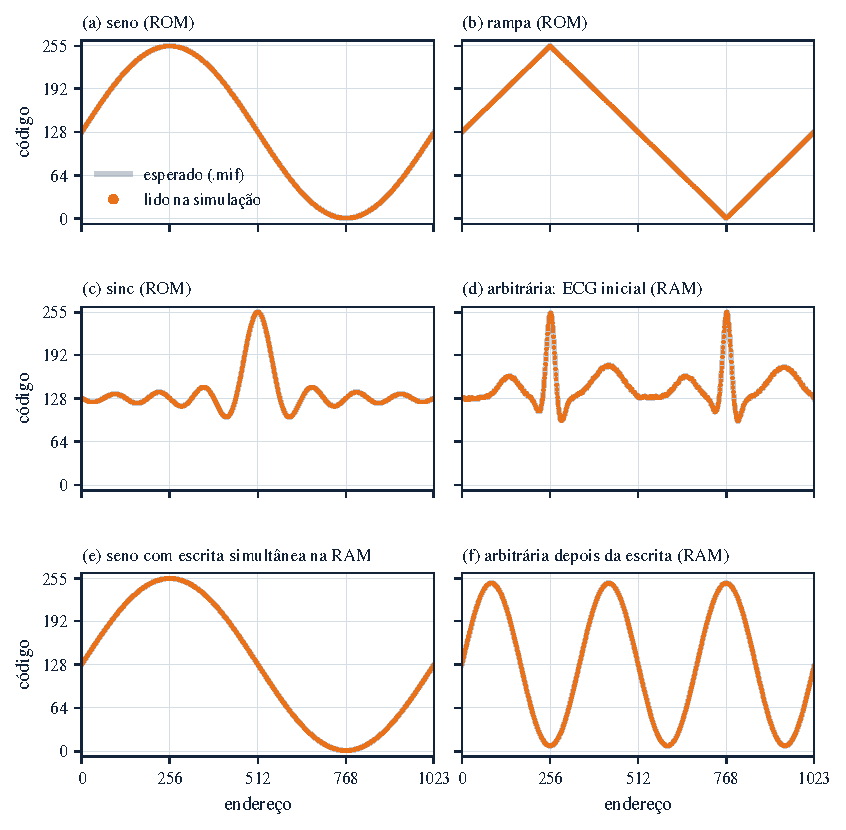
\includegraphics[width=\textwidth]{./figuras/tb_LUT_tabelas}
	\legend{Fonte~---~Autoria própria.}
\end{figure}

\begin{figure}
	\caption{Latência de dois clocks entre o endereço e a amostra nas memórias.}
	\label{fig:tb_lut_lat}
	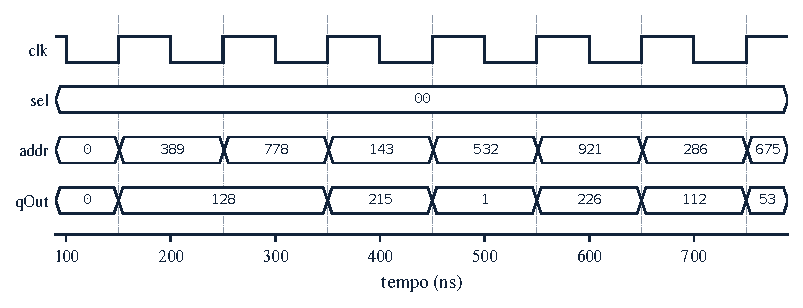
\includegraphics[width=\textwidth]{./figuras/tb_LUT_latencia}
	\legend{Fonte~---~Autoria própria.}
\end{figure}

\subsection{Núcleo DDS}

A Figura~\ref{fig:rtl_core} mostra o núcleo no RTL, com os três blocos ligados em sequência: acumulador de fase, tabelas e registrador de saída.

\begin{figure}
	\caption{Visão RTL do núcleo \acs{dds} (\cod{dds\_core}).}
	\label{fig:rtl_core}
	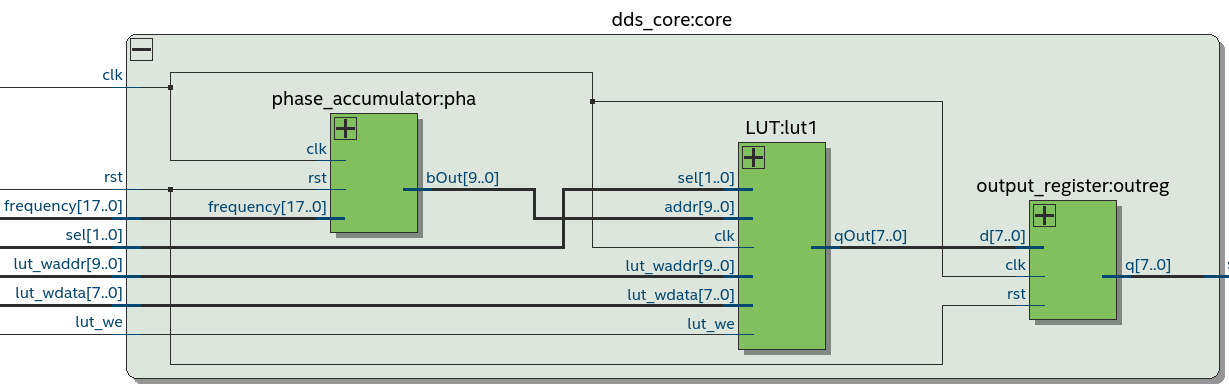
\includegraphics[width=\textwidth]{./figuras/rtl_dds_core}
	\legend{Fonte~---~Autoria própria.}
\end{figure}

O \eng{testbench} do núcleo \cod{dds\_core} comparou 14\,034 amostras de saída com o modelo de referência, sem nenhuma diferença. A Figura~\ref{fig:tb_core} mostra trechos da saída em cada situação testada. Na Figura~\ref{fig:tb_core}(b), a frequência muda de 100~kHz para 262\,143~Hz no instante marcado pela linha tracejada, e o sinal continua sem descontinuidade. Na Figura~\ref{fig:tb_core}(f), a forma de onda é um dente de serra escrito na \ac{ram} enquanto o seno estava na saída.

\begin{figure}
	\caption{Saída do núcleo \acs{dds} para as quatro formas de onda, na troca de frequência e após a escrita da tabela arbitrária.}
	\label{fig:tb_core}
	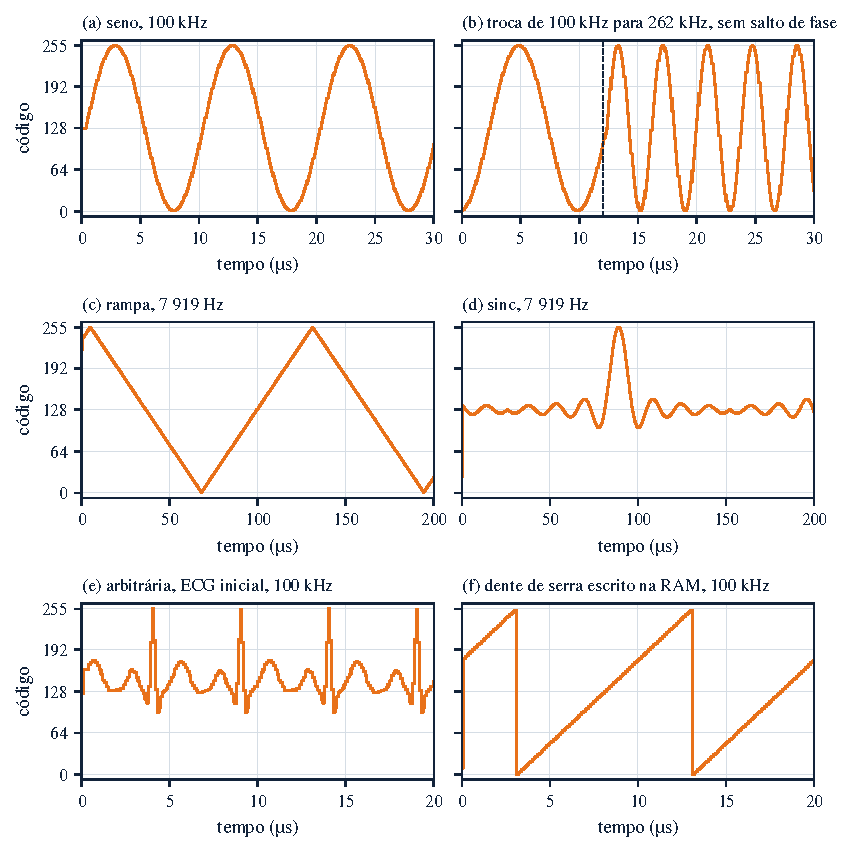
\includegraphics[width=\textwidth]{./figuras/tb_dds_core_formas}
	\legend{Fonte~---~Autoria própria.}
\end{figure}

A Figura~\ref{fig:tb_core_lat} mostra a saída do \eng{reset} em 100~kHz. Durante o \eng{reset}, a amostra permanece em 128, o zero do sinal. Depois dele, o endereço avança 10 posições por clock (\(100~\text{kHz} \cdot 1024/10~\text{MHz} \approx 10{,}24\)), e cada endereço aparece na saída três clocks depois, como previsto.

\begin{figure}
	\caption{Saída do \eng{reset} no núcleo \acs{dds}: latência de três clocks entre o endereço e a amostra.}
	\label{fig:tb_core_lat}
	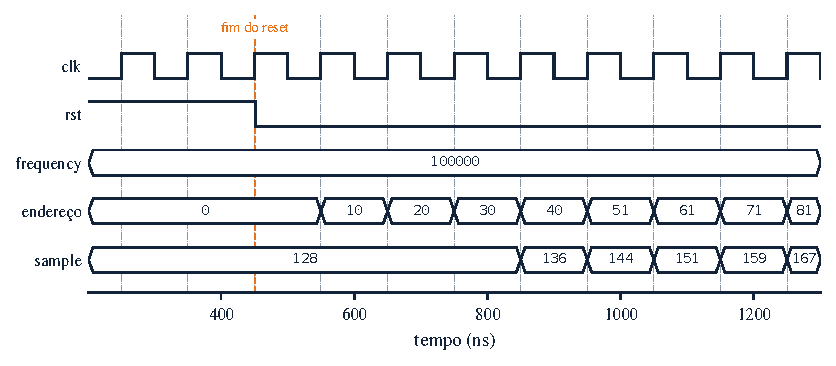
\includegraphics[width=\textwidth]{./figuras/tb_dds_core_latencia}
	\legend{Fonte~---~Autoria própria.}
\end{figure}

\section{Verificação do controle pelo computador}

\pendente{Inserir a visão RTL do \cod{vjtag\_dr} (caminho \cod{pc}, \cod{ctrl}, \cod{dr} no RTL Viewer).}

A Figura~\ref{fig:tb_vjtag} mostra dois comandos de frequência no bloco \cod{vjtag\_dr}. Em cada um, o Capture-DR é seguido de 18 ciclos de Shift-DR, em que os bits entram por \cod{tdi}, com o \ac{lsb} primeiro, e o registrador \cod{dr} se forma. No Update-DR, o valor é copiado para \cod{cmd\_data} e \cod{cmd\_toggle} muda de nível. Durante o segundo deslocamento, \cod{tdo} devolve o valor do primeiro comando (\cod{2A5A5}), carregado no Capture-DR, o que permite ler a configuração.

\begin{figure}
	\caption{Dois comandos de frequência no registrador de dados do Virtual \acs{jtag}.}
	\label{fig:tb_vjtag}
	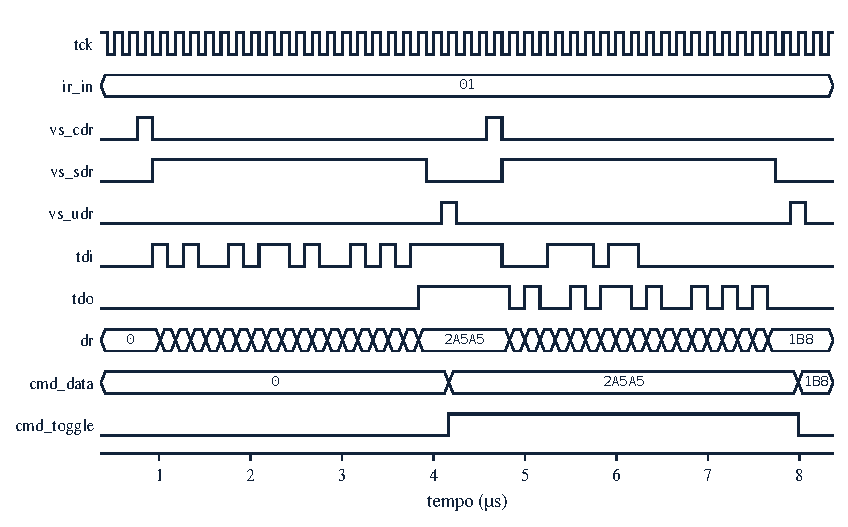
\includegraphics[width=\textwidth]{./figuras/tb_vjtag_dr}
	\legend{Fonte~---~Autoria própria.}
\end{figure}

A Figura~\ref{fig:rtl_cmd_sync} mostra o \cod{cmd\_sync} no RTL: a cadeia de três \eng{flip-flops} do sincronizador (\cod{sync}), o registrador \cod{last}, que guarda o último nível visto, a comparação entre os dois e os registradores de saída \cod{valid} e \cod{data}.

\begin{figure}
	\caption{Visão RTL da passagem de comandos entre domínios de clock (\cod{cmd\_sync}).}
	\label{fig:rtl_cmd_sync}
	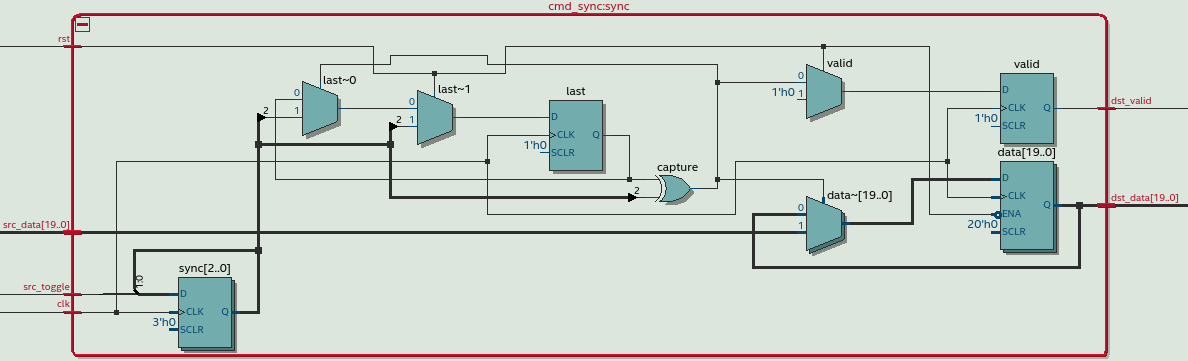
\includegraphics[width=\textwidth]{./figuras/rtl_cmd_sync}
	\legend{Fonte~---~Autoria própria.}
\end{figure}

A Figura~\ref{fig:tb_cmd_sync} mostra a passagem de um comando para o domínio de 10~MHz. A mudança de \cod{src\_toggle} percorre os três \eng{flip-flops} do sincronizador; quando chega ao último, o dado é copiado para \cod{dst\_data} e \cod{dst\_valid} pulsa por um clock. No \eng{testbench}, 300 comandos com dados e intervalos aleatórios, gerados por um clock de 6~MHz sem relação de fase com o de destino, foram entregues uma única vez, em ordem e com o dado correto, e um \eng{reset} no destino não repetiu nenhum comando.

\begin{figure}
	\caption{Passagem de um comando do domínio do \cod{tck} para o de 10~MHz.}
	\label{fig:tb_cmd_sync}
	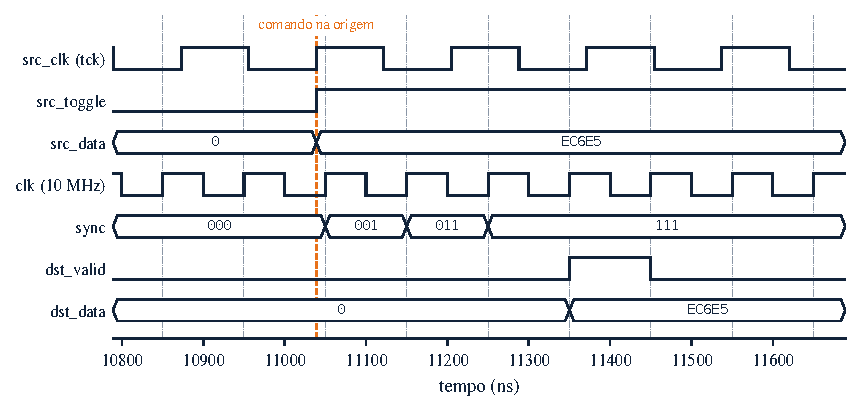
\includegraphics[width=\textwidth]{./figuras/tb_cmd_sync}
	\legend{Fonte~---~Autoria própria.}
\end{figure}

A Figura~\ref{fig:rtl_jtag} mostra o \cod{jtag\_control} no RTL, com os três blocos: \cod{vjtag\_dr}, \cod{cmd\_sync} e \cod{control\_registers}. O comando de 20~bits sai do \cod{vjtag\_dr}, atravessa o \cod{cmd\_sync} e é separado em instrução e dado na entrada dos registradores.

\begin{figure}
	\caption{Visão RTL do controle pelo computador (\cod{jtag\_control}).}
	\label{fig:rtl_jtag}
	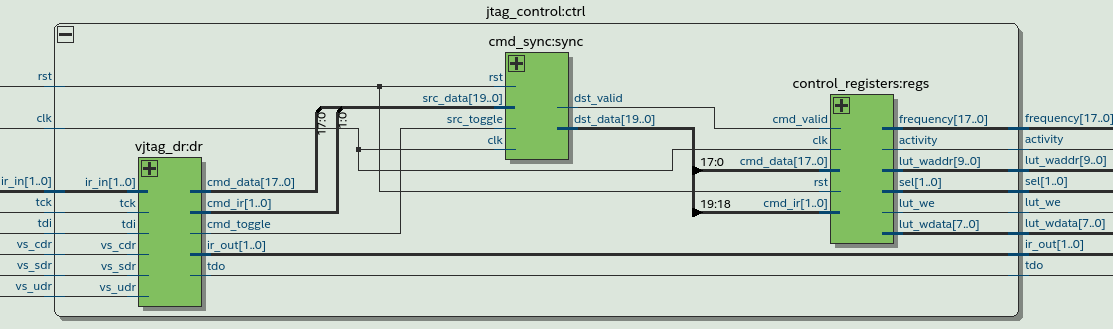
\includegraphics[width=\textwidth]{./figuras/rtl_jtag_control}
	\legend{Fonte~---~Autoria própria.}
\end{figure}

A Figura~\ref{fig:tb_jtag} mostra o caminho completo de um comando de 440~Hz no bloco \cod{jtag\_control}: do deslocamento no domínio do \cod{tck} até o registrador de frequência no domínio de 10~MHz. O registrador é atualizado 566~ns após o Update-DR, um tempo muito menor que o de um novo deslocamento. No mesmo \eng{testbench}, 64 escritas consecutivas na tabela geraram 64 pulsos de escrita, na ordem e com os endereços e dados corretos.

\begin{figure}
	\caption{Comando de frequência do registrador de dados do \acs{jtag} até o registrador de frequência.}
	\label{fig:tb_jtag}
	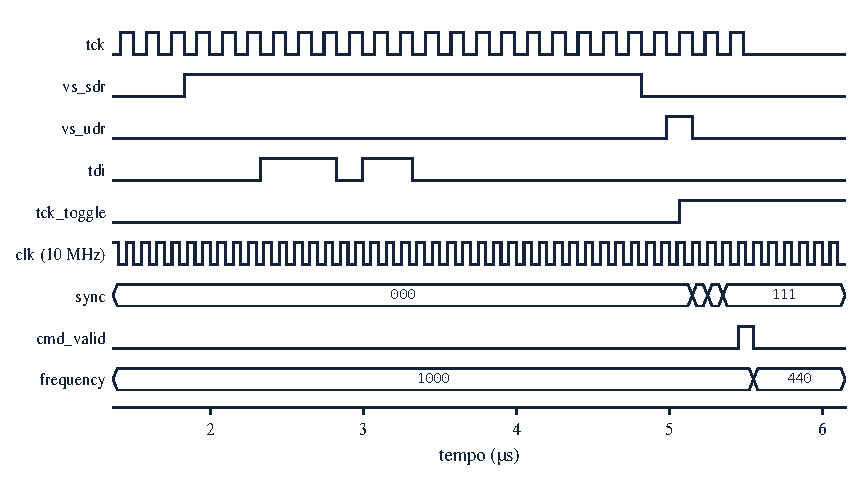
\includegraphics[width=\textwidth]{./figuras/tb_jtag_control}
	\legend{Fonte~---~Autoria própria.}
\end{figure}

\section{Verificação do sistema}

A Figura~\ref{fig:rtl_dds} mostra a entidade do topo no RTL. Ela contém apenas as ligações entre o \ac{pll}, o \cod{reset\_sync}, o \cod{jtag\_interface} e o \cod{dds\_core}, além da porta OU que combina o botão de \eng{reset} com a indicação de travamento do \ac{pll}.

\begin{figure}
	\caption{Visão RTL da entidade do topo (\cod{DDS}).}
	\label{fig:rtl_dds}
	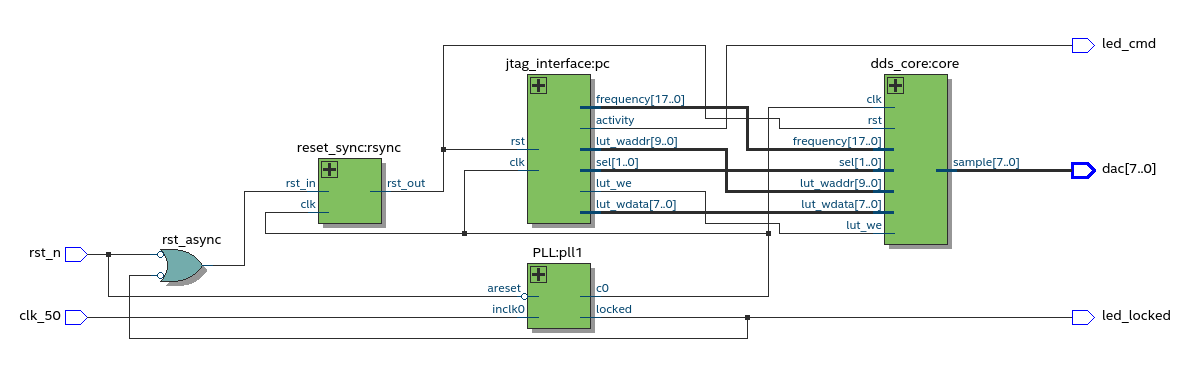
\includegraphics[width=\textwidth]{./figuras/rtl_DDS}
	\legend{Fonte~---~Autoria própria.}
\end{figure}

O \eng{testbench} \cod{tb\_system} reúne o controle e o núcleo e faz o papel do computador, enviando a mesma sequência de comandos que a interface gráfica enviaria. A Figura~\ref{fig:tb_sys} mostra a saída durante toda a simulação. Após o \eng{reset}, sem nenhum comando, o gerador produz o seno de 1~kHz. Em seguida, o computador pede 100~kHz e seno, depois sinc, envia uma tabela inteira, com 1024 escritas, e escolhe a forma arbitrária em 50~kHz. A Figura~\ref{fig:tb_sys_det}(a) mostra o momento em que o comando de frequência chega, e a Figura~\ref{fig:tb_sys_det}(b), a tabela enviada sendo reproduzida. Em cada trecho, cada amostra foi comparada com a tabela correspondente, e a frequência medida pelas voltas do endereço coincidiu com a pedida, dentro da tolerância de 0,1\% usada no \eng{testbench}.

\begin{figure}
	\caption{Saída do sistema durante a sequência de comandos do computador.}
	\label{fig:tb_sys}
	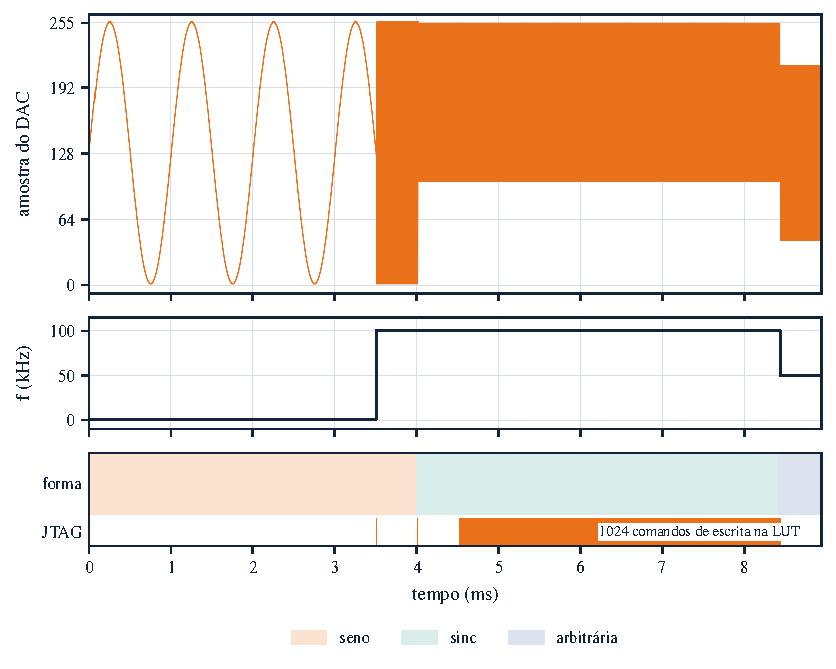
\includegraphics[width=\textwidth]{./figuras/tb_system_visao_geral}
	\legend{Fonte~---~Autoria própria.}
\end{figure}

\begin{figure}
	\caption{Detalhes da simulação do sistema: (a) chegada do comando de frequência; (b) tabela enviada pelo \acs{jtag} reproduzida na saída.}
	\label{fig:tb_sys_det}
	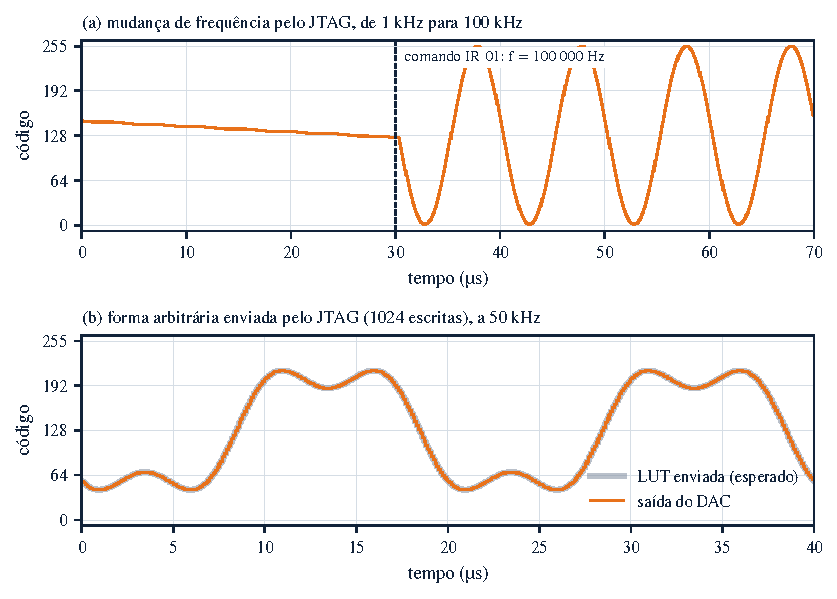
\includegraphics[width=\textwidth]{./figuras/tb_system_detalhes}
	\legend{Fonte~---~Autoria própria.}
\end{figure}

Por fim, o \eng{testbench} \cod{tb\_DDS} simula a entidade do topo, com o \ac{pll} e as memórias pelos modelos da Intel. A Figura~\ref{fig:tb_pll} mostra o travamento do \ac{pll}: o clock de 10~MHz surge, o \eng{LED} de travamento acende e o \eng{reset} interno é liberado três clocks depois. A Figura~\ref{fig:tb_dds} mostra os pinos do \ac{dac}: o seno de 1~kHz após a liberação do botão e o retorno ao código 128 quando o botão é pressionado novamente. A frequência medida nos pinos ficou dentro de 1~Hz de 1~kHz, a tolerância usada no \eng{testbench}.

\begin{figure}
	\caption{Travamento do \acs{pll} e liberação do \eng{reset} interno na entidade do topo.}
	\label{fig:tb_pll}
	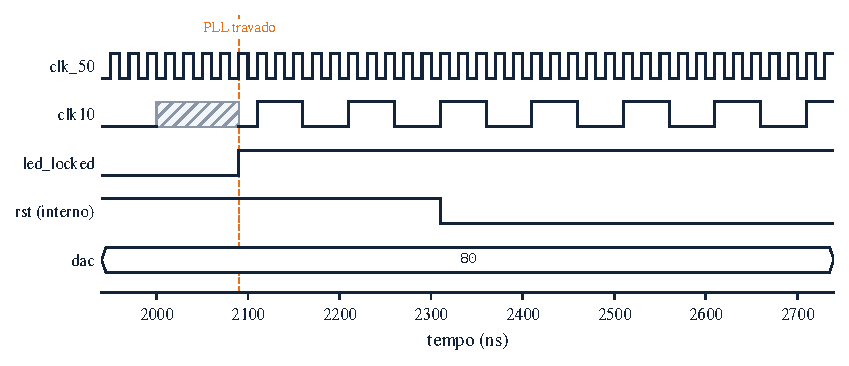
\includegraphics[width=\textwidth]{./figuras/tb_DDS_pll}
	\legend{Fonte~---~Autoria própria.}
\end{figure}

\begin{figure}
	\caption{Código nos pinos do \acs{dac} na simulação da entidade do topo.}
	\label{fig:tb_dds}
	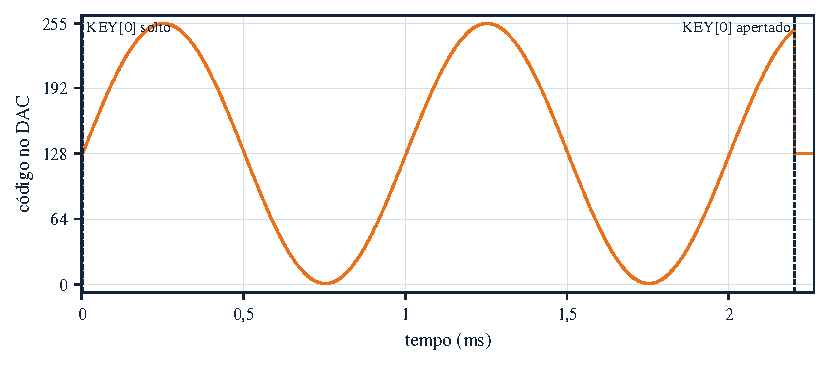
\includegraphics[width=\textwidth]{./figuras/tb_DDS_saida}
	\legend{Fonte~---~Autoria própria.}
\end{figure}

\section{Simulação da placa analógica}

A simulação no LTspice cobre 5~ms, ou cinco períodos do seno de 1~kHz produzido pelo \ac{vhdl}. A Figura~\ref{fig:spice_tempo}(a) mostra a tensão na saída do conversor corrente-tensão e na saída final, depois do ganho, do filtro e do \eng{buffer}; a inversão de fase entre as duas vem do amplificador inversor. A Tabela~\ref{tab:spice} compara os valores obtidos com os calculados no Capítulo~\ref{cap:metodologia}, e todos coincidem. A tensão correspondente ao código 128 não é exatamente zero: como \(I_{FS} = I_{REF} \cdot 255/256\), pela Equação~(\ref{eq:dac0800}), o código 128 dá \(I_{OUT} - \overline{I_{OUT}} = I_{REF}/256\), ou 7,81~mV na saída do conversor.

\begin{table}
	\caption{Valores obtidos na simulação do circuito analógico.}
	\label{tab:spice}
	\begin{tabular}{l c c}\toprule
		Grandeza & Simulado & Calculado\\\midrule
		Corrente de escala completa do \acs{dac} & 1,99~mA & 1,992~mA\\
		Excursão do conversor corrente-tensão & \(-1{,}976\) a \(+1{,}991\)~V & \(-1{,}977\) a \(+1{,}992\)~V\\
		Tensão do código 128 no conversor & 7,81~mV & 7,81~mV\\
		Ganho do estágio inversor & \(-1{,}19999\) & \(-1{,}2\)\\
		Excursão da saída & 4,760~V de pico a pico & 4,763~V de pico a pico\\
		Frequência & 1,000~kHz & 999,998~Hz\\
		Atraso do filtro em 1~kHz & 321~ns & 317~ns\\\bottomrule
	\end{tabular}
	\legend{Fonte~---~Autoria própria.}
\end{table}

A Figura~\ref{fig:spice_tempo}(b) mostra o efeito do filtro de reconstrução em uma subida do seno. Antes do filtro, a saída é uma escada: em 1~kHz, cada código dura cerca de 1~\(\mu\)s e cada degrau tem 18,75~mV, um \ac{lsb} multiplicado pelo ganho. Depois do filtro, as transições ficam suavizadas e atrasadas em 321~ns. Esse atraso concorda com o atraso de grupo de um filtro de segunda ordem em baixa frequência, \(1/(Q\,\omega_0) \approx 317\)~ns, e não depende da forma de onda.

\begin{figure}
	\caption{Simulação da placa analógica para o seno de 1~kHz: (a) saídas do conversor corrente-tensão e do circuito; (b) detalhe de uma subida, antes e depois do filtro.}
	\label{fig:spice_tempo}
	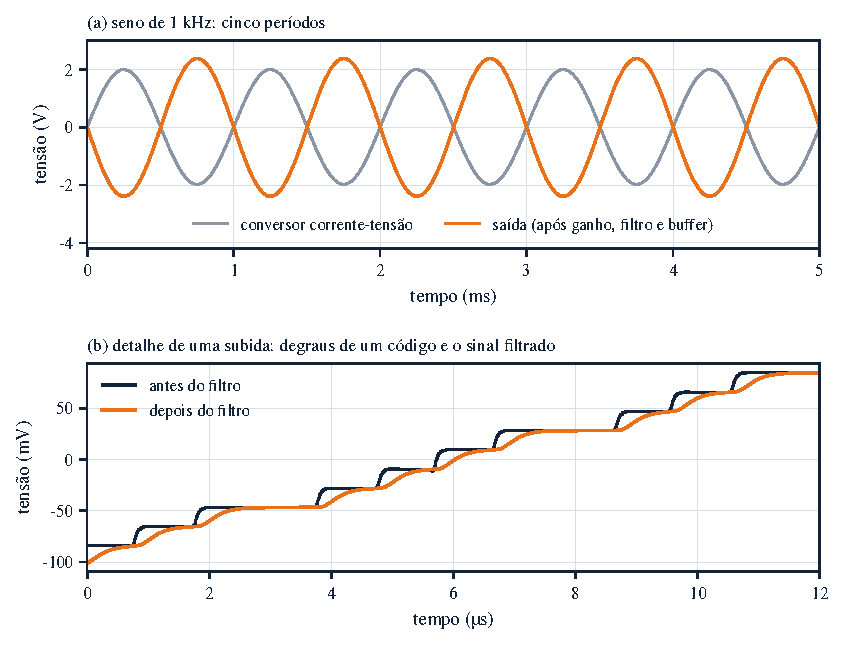
\includegraphics[width=\textwidth]{./figuras/spice_tempo}
	\legend{Fonte~---~Autoria própria.}
\end{figure}

A Figura~\ref{fig:spice_fft} mostra o espectro dos dois pontos, calculado pelo LTspice com resolução de 200~Hz e normalizado pela componente de 1~kHz. Aparecem três grupos de componentes, todos previstos no Capítulo~\ref{cap:teoria}:
\begin{description}
	\item[Harmônicas] --- principalmente ímpares, com a maior, a 9.ª, em \(-73{,}4\)~dBc, e distorção harmônica total, da 2.ª à 10.ª, de \(-70{,}9\)~dBc. Elas vêm da quantização em 8~bits: como o período tem exatamente 1024 amostras, o erro de quantização se repete a cada período e se concentra em harmônicas, em vez de se espalhar como ruído. O filtro não as altera, pois estão dentro da banda passante;
	\item[Imagens da tabela] --- em \(1024 f_{out} \pm f_{out}\) (1,023 e 1,025~MHz). Em 1~kHz, a saída é uma escada de 1024 degraus por período, atualizada a 1,024~MHz, e a Equação~(\ref{eq:zoh}) passa a valer com essa taxa no lugar de \(f_{clk}\). Essa é a maior componente indesejada: \(-60{,}5\)~dBc antes do filtro, em acordo com o limite de \(6{,}02\,P\) da Equação~(\ref{eq:sfdr}), e \(-67{,}0\)~dBc depois, pois o filtro atenua cerca de 6~dB em \(f_0\), como esperado para \(Q = 0{,}5\);
	\item[Imagens do clock] --- em \(f_{clk} \pm f_{out}\), em \(-96\)~dBc antes do filtro e \(-119\)~dBc depois, já próximas do piso numérico da simulação. Nesse ponto, a envoltória sinc da Equação~(\ref{eq:zoh}) vale cerca de \(f_{out}/f_{clk}\), ou \(-80\)~dB, e as transições do \acs{dac} e a banda limitada dos amplificadores atenuam um pouco mais.
\end{description}

\begin{figure}
	\caption{Espectro da simulação da placa analógica para o seno de 1~kHz, antes e depois do filtro de reconstrução.}
	\label{fig:spice_fft}
	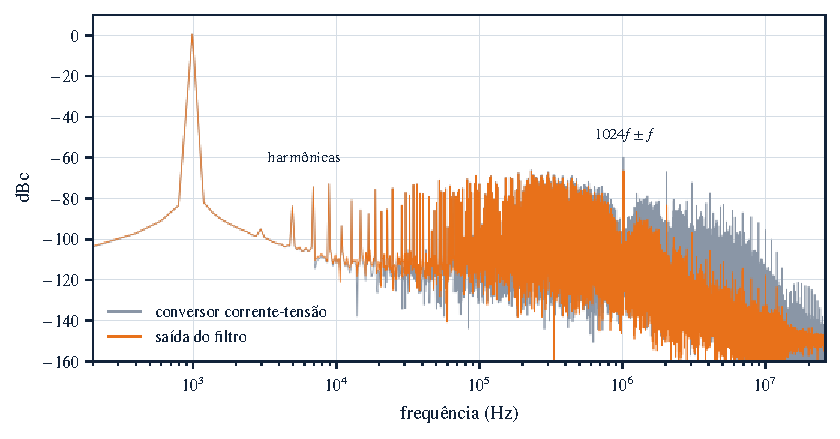
\includegraphics[width=\textwidth]{./figuras/spice_fft}
	\legend{Fonte~---~Autoria própria.}
\end{figure}

\section{Ensaios em bancada}

A Figura~\ref{fig:bancada} mostra a montagem de bancada: a DE2-115, a placa analógica ligada ao conector de expansão, as fontes de \(\pm15\)~V e +10~V e o osciloscópio. Uma medição preliminar da placa analógica, feita em 3 de setembro de 2026 com uma versão anterior do código do \ac{fpga}, é mostrada na Figura~\ref{fig:medicao}: um seno de 100,0~Hz com 5,08~V de pico a pico. \pendente{Confirmar a versão do código usada nessa medição.}

\begin{figure}
	\caption{Montagem de bancada.}
	\label{fig:bancada}
	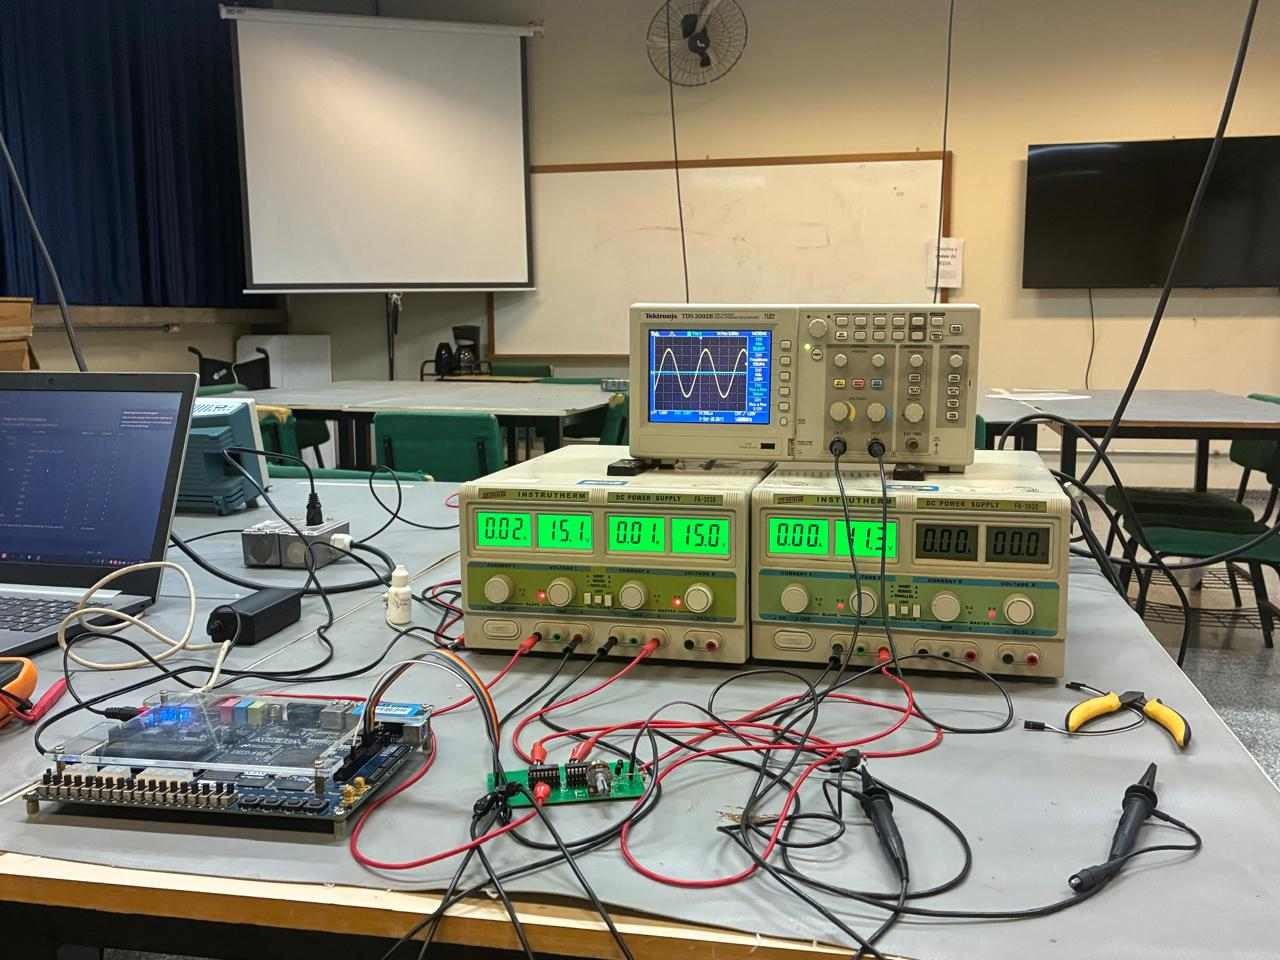
\includegraphics[width=0.8\textwidth]{./figuras/bancada}
	\legend{Fonte~---~Autoria própria.}
\end{figure}

\begin{figure}
	\caption{Medição preliminar na saída da placa analógica: seno de 100,0~Hz com 5,08~V de pico a pico.}
	\label{fig:medicao}
	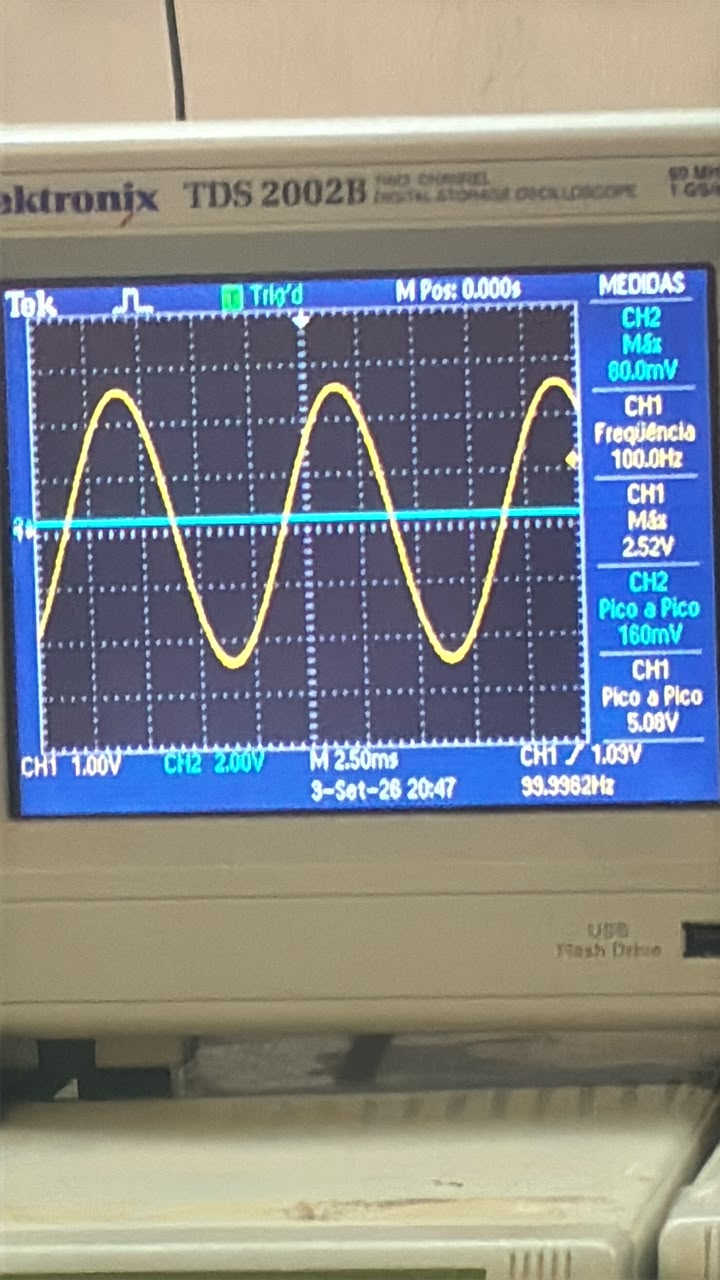
\includegraphics[width=0.5\textwidth]{./figuras/medicao}
	\legend{Fonte~---~Autoria própria.}
\end{figure}

\pendente{Ensaios com o código final: controle pela interface gráfica; frequência medida em vários pontos da faixa; as quatro formas de onda e o envio de uma tabela arbitrária; amplitude e ajuste de ganho; e espectro da saída, para comparar o maior espúrio com a Figura~\ref{fig:espectros}.}

\chapter{Conclusão}\label{cap:conclusao}

Este trabalho desenvolveu um gerador de formas de onda por síntese digital direta, com núcleo em \ac{vhdl} no \ac{fpga} da placa DE2-115, controle pelo computador através do Virtual \ac{jtag}, placa analógica própria e interface gráfica em Python. O gerador produz senoides, rampas, funções sinc e formas arbitrárias de 0 a 262\,143~Hz, com resolução de 2,33~mHz, e dispensa qualquer hardware de comunicação além do cabo de gravação da placa.

O projeto digital foi organizado em blocos encapsulados, com uma entidade por função e um pacote único de constantes. Essa organização permitiu verificar cada bloco isoladamente: os 16 \eng{testbenches} auto-verificáveis, que vão da conversão de frequência à entidade do topo, terminaram sem erros. A separação entre o \ac{ip} do Virtual \ac{jtag} e a lógica de controle permitiu simular o caminho completo, do comando do computador até a amostra no \ac{dac}, que de outra forma só poderia ser verificado na placa. A conversão de frequência por multiplicação em ponto fixo, sem divisor, manteve o erro abaixo de 1~\ac{lsb} da palavra de sintonia em toda a faixa, e a travessia dos comandos entre os domínios de clock, feita com um único bit sincronizado, entregou todos os comandos testados sem perda nem repetição.

O projeto ocupa menos de 1\% dos elementos lógicos do \ac{fpga} e opera com folga de tempo de dez vezes no clock de 10~MHz. A simulação numérica do espectro confirmou que, com tabela de 1024 posições, o maior espúrio de truncamento fica em cerca de \(-60\)~dBc. Assim, o desempenho espectral é limitado principalmente pela resolução de 8~bits do DAC0800.

Na simulação da placa analógica, a saída reproduziu o seno gerado pelo \ac{vhdl} com a amplitude, o ganho e o atraso calculados. A distorção harmônica total foi de \(-70{,}9\)~dBc, e a maior componente indesejada, em \(-67\)~dBc após o filtro, é a imagem associada à resolução da tabela, de acordo com o limite de \(6{,}02\,P\). O estágio de saída classe AB, previsto no projeto da placa, foi retirado por distorção, e a saída passou a ser tomada do seguidor de tensão.

\pendente{Completar com os resultados dos ensaios em bancada com o código final.}

Como trabalhos futuros, propõem-se:
\begin{itemize}
	\item realizar os ensaios em bancada com o código final, medindo a frequência ao longo da faixa e o espectro da saída, para comparar o maior espúrio com o previsto;
	\item comparar a forma de onda e o espectro medidos na placa com os da simulação SPICE;
	\item projetar um estágio de saída com maior capacidade de corrente e baixa distorção, em substituição ao classe AB retirado;
	\item substituir o DAC0800 por um conversor de maior resolução e menor tempo de acomodação, aproveitando a margem de tempo do \ac{fpga} para elevar o clock e a frequência máxima;
	\item usar um filtro de reconstrução de ordem mais alta, para atenuar mais as imagens com a mesma banda passante;
	\item explorar a simetria do seno para reduzir a tabela, liberando memória para tabelas maiores ou para mais formas de onda;
	\item acrescentar modulações (amplitude, frequência e varredura) e um segundo canal com defasagem controlada.
\end{itemize}


%-----------------------------------------------------------------
% ELEMENTOS PÓS-TEXTUAIS
%-----------------------------------------------------------------

\backmatter
\printbibliography

%---
% Apêndices (opcional)
\appendix
\chapter{Organização do repositório}\label{ap:repositorio}
Todos os arquivos do trabalho estão no repositório \url{https://github.com/nseiC/dds_waveform_generator} \cite{seifert2026}, organizados conforme a Tabela~\ref{tab:repositorio}.

\begin{table}[h]
	\caption{Organização do repositório do trabalho.}
	\label{tab:repositorio}
	\begin{tabular}{l p{0.7\textwidth}}\toprule
		Pasta & Conteúdo\\\midrule
		\cod{fpga/} & projeto do Quartus: código \ac{vhdl}, \acp{ip}, tabelas \ac{mif}, pinagem e restrições de tempo\\
		\cod{fpga/testbenches/} & os 16 \eng{testbenches}, o \eng{script} que executa todos e o que desenha as figuras\\
		\cod{GUI/} & interface gráfica em Python e a biblioteca de comunicação pelo Virtual \ac{jtag}\\
		\cod{analog/layout/} & projeto da placa analógica no Altium Designer e arquivos de fabricação\\
		\cod{analog/simulation/} & simulação da placa analógica no LTspice e os estímulos gerados a partir do \ac{vhdl}\\
		\cod{analog/resultados/} & ensaios em bancada: telas, pontos em \ac{csv} e configuração do osciloscópio de cada medida\\
		\cod{docs/} & página interativa da roda de fase e os \eng{scripts} das figuras deste texto\\
		\cod{overleaf/} & este texto\\\bottomrule
	\end{tabular}
	\legend{Fonte~---~Autoria própria.}
\end{table}

Para reproduzir os resultados de simulação, basta executar o \eng{script} \cod{fpga/testbenches/run\_all.sh}, que requer o GHDL e a biblioteca \cod{altera\_mf} do Quartus. As figuras dos \eng{testbenches} são geradas pelo \eng{script} \cod{fpga/testbenches/gerar\_figuras.py}, e as demais figuras deste texto por \cod{docs/gerar\_figuras\_tcc.py}. O projeto do \ac{fpga} é compilado abrindo o arquivo \cod{fpga/DDS.qpf} no Quartus Prime 18.1.

%---

%---
% Anexos (opcional)
%\attachment
%\chapter{Meu anexo}
%O anexo é um elemento pós"-textual opcional contendo elementos que não são da autoria do autor.

%---

%-----------------------------------------------------------------
% FIM DO DOCUMENTO
%-----------------------------------------------------------------

\end{document}
